\documentclass[]{article}
\usepackage{geometry,tikz,lipsum,amsmath,amssymb,soul,xcolor,cancel}
\tikzset{every picture/.style={line width=0.75pt}} %set default line width to 0.75pt        
\numberwithin{equation}{section}

\NewDocumentCommand{\caja}{ m O{gray!40} O{gray!10} m }{
	\begin{figure}[h]
		\centering
		\begin{tikzpicture}
			\node[anchor=text, text width=\columnwidth-1.2cm, draw, rounded corners, line width=1pt, fill=#3, inner sep=5mm] (big) {\\#4};
			\node[draw, rounded corners, line width=.5pt, fill=#2, anchor=west, xshift=5mm] (small) at (big.north west) {#1};
		\end{tikzpicture}
	\end{figure}
}
\NewDocumentCommand{\indUpDown}{ O{\Lambda} O{\mu} O{\nu} }{
	{#1}^{#2}_{\ #3}
}
\NewDocumentCommand{\indDownUp}{ O{\Lambda} O{\mu} O{\nu} }{
	{#1}_{#2}^{\ #3}
}
\newcommand{\LambdaMuNu}{\indUpDown}
\newcommand{\0}{\textcolor{gray}{0}}

%opening
\title{Mecánica Clásica Avanzada}
\author{Simon Fonseca}

\begin{document}

\maketitle


\section{Teoría de la Relatividad Especial}
\subsection{Transformaciones de Galileo}

\caja{Sistema de referencia}{Sistema de coordenadas que sirve para indicar la posición de una partícula en el espacio, junto con un "reloj" fijado al sistema para indicar el tiempo.}

\caja{Sistema de referencia \textbf{inercial}}{Un sistema donde un objeto sobre el cual no se ejercen fuerzas externas se mueve a velocidad constante. En otras palabras, un sistema que no está acelerando ni rotando.} 
\begin{figure}
	\centering
	\begin{tikzpicture}[x=0.75pt,y=0.75pt,yscale=-1,xscale=1]
		%uncomment if require: \path (0,281); %set diagram left start at 0, and has height of 281
		
		%Straight Lines [id:da5753987644902085] 
		\draw    (0,251.49) -- (77.85,193.45) ;
		%Shape: Right Angle [id:dp4524626209936883] 
		\draw   (229.95,193.45) -- (77.85,193.45) -- (77.85,43.68) ;
		
		%Straight Lines [id:da15588215025867458] 
		\draw    (120,213.17) -- (197.85,155.13) ;
		%Shape: Right Angle [id:dp35424357388621874] 
		\draw   (349.95,155.13) -- (197.85,155.13) -- (197.85,5.36) ;
		
		%Straight Lines [id:da3815965393266346] 
		\draw    (250.5,137.75) -- (298.5,137.75) ;
		\draw [shift={(300.5,137.75)}, rotate = 180] [color={rgb, 255:red, 0; green, 0; blue, 0 }  ][line width=0.75]    (10.93,-3.29) .. controls (6.95,-1.4) and (3.31,-0.3) .. (0,0) .. controls (3.31,0.3) and (6.95,1.4) .. (10.93,3.29)   ;
		
		% Text Node
		\draw (56.62,40.32) node [anchor=north west][inner sep=0.75pt]   [align=left] {$\displaystyle x_{1}$$ $};
		% Text Node
		\draw (15.65,240) node [anchor=north west][inner sep=0.75pt]   [align=left] {$\displaystyle x_{2}$$ $};
		% Text Node
		\draw (206,200) node [anchor=north west][inner sep=0.75pt]   [align=left] {$\displaystyle x_{3}$$ $};
		% Text Node
		\draw (58.19,179.73) node [anchor=north west][inner sep=0.75pt]   [align=left] {$\displaystyle O$};
		% Text Node
		\draw (86,112) node [anchor=north west][inner sep=0.75pt]   [align=left] {$\displaystyle K$};
		% Text Node
		\draw (269.75,115.5) node [anchor=north west][inner sep=0.75pt]   [align=left] {$\displaystyle \vec{V}$};
		% Text Node
		\draw (176.62,2) node [anchor=north west][inner sep=0.75pt]   [align=left] {$\displaystyle x'_{1}$$ $};
		% Text Node
		\draw (135.65,201.68) node [anchor=north west][inner sep=0.75pt]   [align=left] {$\displaystyle x'_{2}$$ $};
		% Text Node
		\draw (326,160) node [anchor=north west][inner sep=0.75pt]   [align=left] {$\displaystyle x'_{3}$$ $};
		% Text Node
		\draw (178.22,141.41) node [anchor=north west][inner sep=0.75pt]   [align=left] {$\displaystyle O'$};
		% Text Node
		\draw (208,72) node [anchor=north west][inner sep=0.75pt]   [align=left] {$\displaystyle K'$};
		
	\end{tikzpicture}
\end{figure}

\caja{Invariante}{Un objeto o concepto es invariante cuando no cambia bajo ninguna transformación (Ejemplos newtonianos: masa, distancia, intervalo temporal).}

\caja{Ecuación covariante}{Una ecuación es covariante cuando, bajo cualquier transformación, sus elementos cambian pero la relación se mantiene idéntica (Ej: $\mathbf{F}=m\mathbf{a} \Leftrightarrow \mathbf{F}'=m\mathbf{a}'$, los elementos vectoriales de $\mathbf{F}$ y $\mathbf{a}$ cambiaron, pero la estructura de la ecuación se mantiene).}

Si tenemos dos sistemas de referencia $K$ y $K'$, podemos encontrar ecuaciones de transformación que relacionen las coordenadas en $K$ ($t, \mathbf{x}, \mathbf{v}$) a las coordenadas en $K'$ ($t', \mathbf{x}', \mathbf{v}'$). En mecánica newtoniana, se cumple que:
\begin{itemize}
	\item Todos los sistemas inerciales son equivalentes, todas las leyes físicas son idénticas sin importar su sistema. En otras palabras, las ecuaciones son invariantes con respecto a transformaciones entre sistemas inerciales.
	\item El tiempo es absoluto.
	\begin{equation}
		t' = t
	\end{equation}
	\item Transformación de coordenadas, distancias, velocidades y fuerzas entre dos sistemas  $K$ y $K'$, donde $K'$ se mueve a la derecha en relación a $K$ con velocidad constante $\mathbf{V}$:
	\begin{align*}
		\mathbf{x}' &= \mathbf{x} - \mathbf{V}t \\
		\Delta\mathbf{x}' &= \Delta\mathbf{x} \\
		\mathbf{v}' &= \mathbf{v} - \mathbf{V} \\
		\mathbf{F}' &= \mathbf{F} 
	\end{align*}
	\item Las interacciones entre dos partículas son instantáneas (Ej: Si el Sol desaparece, la Tierra saldrá disparada inmediatamente). 
\end{itemize}

Si definimos convenientemente los ejes, tal que $X$ y $X'$ coincidan consigo mismo y con la dirección de movimiento de $K'$, y los ejes $Y$, $Z$ paralelos a $Y$, $Z$, obtendremos las \textbf{transformaciones de Galileo}:
\begin{align}
	x&=x'+Vt\\
	y&=y'\\
	z&=z'\\
	t&=t'
\end{align}

Pero en el siglo XIX, la ecuaciones de Maxwell contradijeron el principio galileano de covarianza. Si tomamos el campo eléctrico de una partícula cargada $q$ en un marco inercial:
\begin{equation*}
	\Rightarrow  \mathbf{E} = \frac{q}{4\pi\epsilon_0}\frac{\mathbf{\hat{r}}}{r^2}
\end{equation*}
Y aplicamos una transformación:
\begin{align*}
	\mathbf{x}' &= x - \mathbf{V}t \\
	\Rightarrow \nabla &= \nabla' \\
	\Rightarrow \frac{\partial}{\partial t} &= \frac{\partial}{\partial t'} - (\mathbf{V}\cdot\nabla')
\end{align*}
Podemos ver que la ecuación de onda electromagnética:
\begin{equation}
	\frac{1}{c^2}\frac{\partial^2\mathbf{E}}{\partial t^2} = \nabla^2\mathbf{E} \Leftrightarrow \frac{1}{c^2}\left(\frac{\partial^2\mathbf{E}'}{\partial t'^2} - 2(\mathbf{V}\cdot\nabla')\frac{\partial\mathbf{E}'}{\partial t'} + (\mathbf{V}\cdot\nabla')^2\mathbf{E}'\right)  = \nabla'^2\mathbf{E}'
	\label{eqn:onda_transformada_galileo}
\end{equation}
Por lo tanto, la ecuación de onda no es covariante. El mismo resultado se obtiene al considerar la ecuación de onda acústica. Los físicos del siglo XIX esperaban entonces que, al igual que el sonido al aire, la luz tuviera un medio por el cual se moviera y en el cual su ecuación de onda fuera "limpia" (como la del lado izquierdo de \ref{eqn:onda_transformada_galileo}). A este medio de luz se le llamo \textbf{ether}.

\subsection{Experimentos de Michelson y Morley}
Para probar la existencia del "viento de ether", Michelson y Morley desarrollaron un experimento en el que, si la teoría era correcta, sería capaz de detectar cambios en la interferencia de dos haces de luz dependiendo de la estación del año.
\begin{figure}
	\centering
	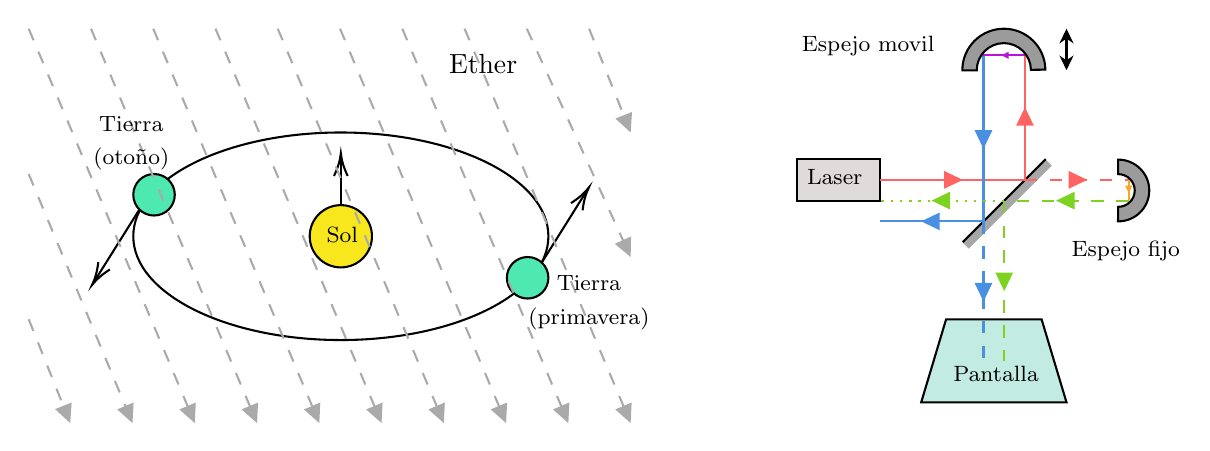
\begin{tikzpicture}[x=0.75pt,y=0.75pt,yscale=-1,xscale=1]
		%uncomment if require: \path (0,300); %set diagram left start at 0, and has height of 300
		
		%Shape: Trapezoid [id:dp296737940988709] 
		\draw  [fill={rgb, 255:red, 194; green, 235; blue, 226 }  ,fill opacity=1 ] (460,200) -- (472,160) -- (518,160) -- (530,200) -- cycle ;
		%Straight Lines [id:da5920030990100863] 
		\draw [color={rgb, 255:red, 167; green, 167; blue, 167 }  ,draw opacity=1 ][fill={rgb, 255:red, 179; green, 179; blue, 179 }  ,fill opacity=1 ][line width=3]    (481.5,124.57) -- (521.5,84.57) ;
		%Straight Lines [id:da41121562255159383] 
		\draw    (480,122.82) -- (520,82.82) ;
		
		%Straight Lines [id:da9685201719421942] 
		\draw    (180.38,120) -- (180.38,82) ;
		\draw [shift={(180.38,80)}, rotate = 90] [color={rgb, 255:red, 0; green, 0; blue, 0 }  ][line width=0.75]    (10.93,-3.29) .. controls (6.95,-1.4) and (3.31,-0.3) .. (0,0) .. controls (3.31,0.3) and (6.95,1.4) .. (10.93,3.29)   ;
		%Shape: Ellipse [id:dp6583363609039639] 
		\draw   (80.38,120) .. controls (80.38,92.39) and (125.15,70) .. (180.38,70) .. controls (235.6,70) and (280.38,92.39) .. (280.38,120) .. controls (280.38,147.61) and (235.6,170) .. (180.38,170) .. controls (125.15,170) and (80.38,147.61) .. (80.38,120) -- cycle ;
		%Shape: Circle [id:dp7559209954289742] 
		\draw  [fill={rgb, 255:red, 248; green, 231; blue, 28 }  ,fill opacity=1 ] (165.38,120) .. controls (165.38,111.72) and (172.09,105) .. (180.38,105) .. controls (188.66,105) and (195.38,111.72) .. (195.38,120) .. controls (195.38,128.28) and (188.66,135) .. (180.38,135) .. controls (172.09,135) and (165.38,128.28) .. (165.38,120) -- cycle ;
		%Shape: Circle [id:dp44889698088513164] 
		\draw  [fill={rgb, 255:red, 77; green, 233; blue, 177 }  ,fill opacity=1 ] (80.38,100) .. controls (80.38,94.48) and (84.85,90) .. (90.38,90) .. controls (95.9,90) and (100.38,94.48) .. (100.38,100) .. controls (100.38,105.52) and (95.9,110) .. (90.38,110) .. controls (84.85,110) and (80.38,105.52) .. (80.38,100) -- cycle ;
		%Shape: Circle [id:dp789775749385696] 
		\draw  [fill={rgb, 255:red, 77; green, 233; blue, 177 }  ,fill opacity=1 ] (260.38,140) .. controls (260.38,134.48) and (264.85,130) .. (270.38,130) .. controls (275.9,130) and (280.38,134.48) .. (280.38,140) .. controls (280.38,145.52) and (275.9,150) .. (270.38,150) .. controls (264.85,150) and (260.38,145.52) .. (260.38,140) -- cycle ;
		%Straight Lines [id:da6676714414388956] 
		\draw    (83.25,107.25) -- (61.56,141.81) ;
		\draw [shift={(60.5,143.5)}, rotate = 302.11] [color={rgb, 255:red, 0; green, 0; blue, 0 }  ][line width=0.75]    (10.93,-3.29) .. controls (6.95,-1.4) and (3.31,-0.3) .. (0,0) .. controls (3.31,0.3) and (6.95,1.4) .. (10.93,3.29)   ;
		%Straight Lines [id:da03515298295129565] 
		\draw    (298.81,98.19) -- (277.13,132.75) ;
		\draw [shift={(299.88,96.5)}, rotate = 122.11] [color={rgb, 255:red, 0; green, 0; blue, 0 }  ][line width=0.75]    (10.93,-3.29) .. controls (6.95,-1.4) and (3.31,-0.3) .. (0,0) .. controls (3.31,0.3) and (6.95,1.4) .. (10.93,3.29)   ;
		%Straight Lines [id:da7335320052735711] 
		\draw [color={rgb, 255:red, 170; green, 170; blue, 170 }  ,draw opacity=1 ] [dash pattern={on 4.5pt off 4.5pt}]  (30,20) -- (108.84,207.24) ;
		\draw [shift={(110,210)}, rotate = 247.17] [fill={rgb, 255:red, 170; green, 170; blue, 170 }  ,fill opacity=1 ][line width=0.08]  [draw opacity=0] (8.93,-4.29) -- (0,0) -- (8.93,4.29) -- cycle    ;
		%Straight Lines [id:da30495065590265524] 
		\draw [color={rgb, 255:red, 170; green, 170; blue, 170 }  ,draw opacity=1 ] [dash pattern={on 4.5pt off 4.5pt}]  (60,20) -- (138.84,207.24) ;
		\draw [shift={(140,210)}, rotate = 247.17] [fill={rgb, 255:red, 170; green, 170; blue, 170 }  ,fill opacity=1 ][line width=0.08]  [draw opacity=0] (8.93,-4.29) -- (0,0) -- (8.93,4.29) -- cycle    ;
		%Straight Lines [id:da0076661913263330606] 
		\draw [color={rgb, 255:red, 170; green, 170; blue, 170 }  ,draw opacity=1 ] [dash pattern={on 4.5pt off 4.5pt}]  (90,20) -- (168.84,207.24) ;
		\draw [shift={(170,210)}, rotate = 247.17] [fill={rgb, 255:red, 170; green, 170; blue, 170 }  ,fill opacity=1 ][line width=0.08]  [draw opacity=0] (8.93,-4.29) -- (0,0) -- (8.93,4.29) -- cycle    ;
		%Straight Lines [id:da18189940989954934] 
		\draw [color={rgb, 255:red, 170; green, 170; blue, 170 }  ,draw opacity=1 ] [dash pattern={on 4.5pt off 4.5pt}]  (120,20) -- (198.84,207.24) ;
		\draw [shift={(200,210)}, rotate = 247.17] [fill={rgb, 255:red, 170; green, 170; blue, 170 }  ,fill opacity=1 ][line width=0.08]  [draw opacity=0] (8.93,-4.29) -- (0,0) -- (8.93,4.29) -- cycle    ;
		%Straight Lines [id:da6247937802786642] 
		\draw [color={rgb, 255:red, 170; green, 170; blue, 170 }  ,draw opacity=1 ] [dash pattern={on 4.5pt off 4.5pt}]  (150,20) -- (228.84,207.24) ;
		\draw [shift={(230,210)}, rotate = 247.17] [fill={rgb, 255:red, 170; green, 170; blue, 170 }  ,fill opacity=1 ][line width=0.08]  [draw opacity=0] (8.93,-4.29) -- (0,0) -- (8.93,4.29) -- cycle    ;
		%Straight Lines [id:da35283850373920067] 
		\draw [color={rgb, 255:red, 170; green, 170; blue, 170 }  ,draw opacity=1 ] [dash pattern={on 4.5pt off 4.5pt}]  (180,20) -- (258.84,207.24) ;
		\draw [shift={(260,210)}, rotate = 247.17] [fill={rgb, 255:red, 170; green, 170; blue, 170 }  ,fill opacity=1 ][line width=0.08]  [draw opacity=0] (8.93,-4.29) -- (0,0) -- (8.93,4.29) -- cycle    ;
		%Straight Lines [id:da5655926894548295] 
		\draw [color={rgb, 255:red, 170; green, 170; blue, 170 }  ,draw opacity=1 ] [dash pattern={on 4.5pt off 4.5pt}]  (210,20) -- (288.84,207.24) ;
		\draw [shift={(290,210)}, rotate = 247.17] [fill={rgb, 255:red, 170; green, 170; blue, 170 }  ,fill opacity=1 ][line width=0.08]  [draw opacity=0] (8.93,-4.29) -- (0,0) -- (8.93,4.29) -- cycle    ;
		%Straight Lines [id:da3346640616133051] 
		\draw [color={rgb, 255:red, 170; green, 170; blue, 170 }  ,draw opacity=1 ] [dash pattern={on 4.5pt off 4.5pt}]  (30,90) -- (78.85,207.23) ;
		\draw [shift={(80,210)}, rotate = 247.38] [fill={rgb, 255:red, 170; green, 170; blue, 170 }  ,fill opacity=1 ][line width=0.08]  [draw opacity=0] (8.93,-4.29) -- (0,0) -- (8.93,4.29) -- cycle    ;
		%Straight Lines [id:da7508733161904289] 
		\draw [color={rgb, 255:red, 170; green, 170; blue, 170 }  ,draw opacity=1 ] [dash pattern={on 4.5pt off 4.5pt}]  (240,20) -- (318.84,207.24) ;
		\draw [shift={(320,210)}, rotate = 247.17] [fill={rgb, 255:red, 170; green, 170; blue, 170 }  ,fill opacity=1 ][line width=0.08]  [draw opacity=0] (8.93,-4.29) -- (0,0) -- (8.93,4.29) -- cycle    ;
		%Straight Lines [id:da07570286845102803] 
		\draw [color={rgb, 255:red, 170; green, 170; blue, 170 }  ,draw opacity=1 ] [dash pattern={on 4.5pt off 4.5pt}]  (270,20) -- (318.76,127.27) ;
		\draw [shift={(320,130)}, rotate = 245.56] [fill={rgb, 255:red, 170; green, 170; blue, 170 }  ,fill opacity=1 ][line width=0.08]  [draw opacity=0] (8.93,-4.29) -- (0,0) -- (8.93,4.29) -- cycle    ;
		%Straight Lines [id:da9909092416778857] 
		\draw [color={rgb, 255:red, 170; green, 170; blue, 170 }  ,draw opacity=1 ] [dash pattern={on 4.5pt off 4.5pt}]  (30,160) -- (48.89,207.21) ;
		\draw [shift={(50,210)}, rotate = 248.2] [fill={rgb, 255:red, 170; green, 170; blue, 170 }  ,fill opacity=1 ][line width=0.08]  [draw opacity=0] (8.93,-4.29) -- (0,0) -- (8.93,4.29) -- cycle    ;
		%Straight Lines [id:da5159021606779878] 
		\draw [color={rgb, 255:red, 170; green, 170; blue, 170 }  ,draw opacity=1 ] [dash pattern={on 4.5pt off 4.5pt}]  (300,20) -- (318.89,67.21) ;
		\draw [shift={(320,70)}, rotate = 248.2] [fill={rgb, 255:red, 170; green, 170; blue, 170 }  ,fill opacity=1 ][line width=0.08]  [draw opacity=0] (8.93,-4.29) -- (0,0) -- (8.93,4.29) -- cycle    ;
		%Shape: Rectangle [id:dp5505953988324193] 
		\draw  [fill={rgb, 255:red, 224; green, 219; blue, 219 }  ,fill opacity=1 ] (400,82.82) -- (440,82.82) -- (440,102.82) -- (400,102.82) -- cycle ;
		%Straight Lines [id:da42064532788750797] 
		\draw [color={rgb, 255:red, 255; green, 100; blue, 100 }  ,draw opacity=1 ]   (440,92.82) -- (510,92.82) ;
		\draw [shift={(480,92.82)}, rotate = 180] [fill={rgb, 255:red, 255; green, 100; blue, 100 }  ,fill opacity=1 ][line width=0.08]  [draw opacity=0] (8.93,-4.29) -- (0,0) -- (8.93,4.29) -- cycle    ;
		%Straight Lines [id:da5282493244177981] 
		\draw [color={rgb, 255:red, 255; green, 100; blue, 100 }  ,draw opacity=1 ]   (510,92.82) -- (510,32.82) ;
		\draw [shift={(510,57.82)}, rotate = 90] [fill={rgb, 255:red, 255; green, 100; blue, 100 }  ,fill opacity=1 ][line width=0.08]  [draw opacity=0] (8.93,-4.29) -- (0,0) -- (8.93,4.29) -- cycle    ;
		%Straight Lines [id:da6568775705414689] 
		\draw [color={rgb, 255:red, 255; green, 100; blue, 100 }  ,draw opacity=1 ] [dash pattern={on 4.5pt off 4.5pt}]  (510,92.82) -- (560,92.82) ;
		\draw [shift={(540,92.82)}, rotate = 180] [fill={rgb, 255:red, 255; green, 100; blue, 100 }  ,fill opacity=1 ][line width=0.08]  [draw opacity=0] (8.93,-4.29) -- (0,0) -- (8.93,4.29) -- cycle    ;
		%Straight Lines [id:da8268928753947329] 
		\draw [color={rgb, 255:red, 74; green, 144; blue, 226 }  ,draw opacity=1 ]   (490,32.82) -- (490,112.82) ;
		\draw [shift={(490,77.82)}, rotate = 270] [fill={rgb, 255:red, 74; green, 144; blue, 226 }  ,fill opacity=1 ][line width=0.08]  [draw opacity=0] (8.93,-4.29) -- (0,0) -- (8.93,4.29) -- cycle    ;
		%Straight Lines [id:da08414389145045498] 
		\draw [color={rgb, 255:red, 126; green, 211; blue, 33 }  ,draw opacity=1 ] [dash pattern={on 4.5pt off 4.5pt}]  (560,102.82) -- (500,102.82) ;
		\draw [shift={(525,102.82)}, rotate = 360] [fill={rgb, 255:red, 126; green, 211; blue, 33 }  ,fill opacity=1 ][line width=0.08]  [draw opacity=0] (8.93,-4.29) -- (0,0) -- (8.93,4.29) -- cycle    ;
		%Straight Lines [id:da3533061152216377] 
		\draw [color={rgb, 255:red, 126; green, 211; blue, 33 }  ,draw opacity=1 ] [dash pattern={on 0.84pt off 2.51pt}]  (500,102.82) -- (440,102.82) ;
		\draw [shift={(465,102.82)}, rotate = 360] [fill={rgb, 255:red, 126; green, 211; blue, 33 }  ,fill opacity=1 ][line width=0.08]  [draw opacity=0] (8.93,-4.29) -- (0,0) -- (8.93,4.29) -- cycle    ;
		%Straight Lines [id:da1545803117361455] 
		\draw [color={rgb, 255:red, 74; green, 144; blue, 226 }  ,draw opacity=1 ] [dash pattern={on 4.5pt off 4.5pt}]  (490,112.82) -- (490,180) ;
		\draw [shift={(490,151.41)}, rotate = 270] [fill={rgb, 255:red, 74; green, 144; blue, 226 }  ,fill opacity=1 ][line width=0.08]  [draw opacity=0] (8.93,-4.29) -- (0,0) -- (8.93,4.29) -- cycle    ;
		%Straight Lines [id:da18426244243489642] 
		\draw [color={rgb, 255:red, 126; green, 211; blue, 33 }  ,draw opacity=1 ] [dash pattern={on 4.5pt off 4.5pt}]  (500,102.82) -- (500,180) ;
		\draw [shift={(500,146.41)}, rotate = 270] [fill={rgb, 255:red, 126; green, 211; blue, 33 }  ,fill opacity=1 ][line width=0.08]  [draw opacity=0] (8.93,-4.29) -- (0,0) -- (8.93,4.29) -- cycle    ;
		%Straight Lines [id:da76557841684744] 
		\draw [color={rgb, 255:red, 74; green, 144; blue, 226 }  ,draw opacity=1 ]   (490,112.82) -- (440,112.82) ;
		\draw [shift={(460,112.82)}, rotate = 360] [fill={rgb, 255:red, 74; green, 144; blue, 226 }  ,fill opacity=1 ][line width=0.08]  [draw opacity=0] (8.93,-4.29) -- (0,0) -- (8.93,4.29) -- cycle    ;
		%Straight Lines [id:da5650779325951993] 
		\draw [color={rgb, 255:red, 189; green, 16; blue, 224 }  ,draw opacity=1 ]   (510,32.82) -- (490,32.82) ;
		\draw [shift={(498.6,32.82)}, rotate = 360] [fill={rgb, 255:red, 189; green, 16; blue, 224 }  ,fill opacity=1 ][line width=0.08]  [draw opacity=0] (3.57,-1.72) -- (0,0) -- (3.57,1.72) -- cycle    ;
		%Shape: Block Arc [id:dp24061981909252805] 
		\draw  [fill={rgb, 255:red, 155; green, 155; blue, 155 }  ,fill opacity=1 ] (479.82,40.06) .. controls (479.82,40.04) and (479.82,40.02) .. (479.82,40) .. controls (479.82,28.95) and (488.77,20) .. (499.82,20) .. controls (510.77,20) and (519.67,28.8) .. (519.82,39.72) -- (512.87,39.82) .. controls (512.78,32.69) and (506.97,26.94) .. (499.82,26.94) .. controls (492.61,26.94) and (486.76,32.79) .. (486.76,40) .. controls (486.76,40.01) and (486.76,40.03) .. (486.76,40.04) -- cycle ;
		%Shape: Block Arc [id:dp963782832071332] 
		\draw  [fill={rgb, 255:red, 155; green, 155; blue, 155 }  ,fill opacity=1 ] (554.89,83.07) .. controls (554.91,83.07) and (554.92,83.07) .. (554.94,83.07) .. controls (563.19,83.07) and (569.88,89.73) .. (569.88,97.94) .. controls (569.88,106.16) and (563.19,112.82) .. (554.94,112.82) .. controls (554.9,112.82) and (554.86,112.82) .. (554.82,112.82) -- (554.88,105.82) .. controls (554.9,105.82) and (554.92,105.82) .. (554.94,105.82) .. controls (559.32,105.82) and (562.88,102.29) .. (562.88,97.94) .. controls (562.88,93.59) and (559.32,90.07) .. (554.94,90.07) .. controls (554.93,90.07) and (554.92,90.07) .. (554.91,90.07) -- cycle ;
		%Straight Lines [id:da44626714375838983] 
		\draw [color={rgb, 255:red, 245; green, 166; blue, 35 }  ,draw opacity=1 ]   (560,92.82) -- (560,102.82) ;
		\draw [shift={(560,99.22)}, rotate = 270] [fill={rgb, 255:red, 245; green, 166; blue, 35 }  ,fill opacity=1 ][line width=0.08]  [draw opacity=0] (3.57,-1.72) -- (0,0) -- (3.57,1.72) -- cycle    ;
		%Straight Lines [id:da2782331932925022] 
		\draw    (530,23) -- (530,37) ;
		\draw [shift={(530,40)}, rotate = 270] [fill={rgb, 255:red, 0; green, 0; blue, 0 }  ][line width=0.08]  [draw opacity=0] (7.14,-3.43) -- (0,0) -- (7.14,3.43) -- (4.74,0) -- cycle    ;
		\draw [shift={(530,20)}, rotate = 90] [fill={rgb, 255:red, 0; green, 0; blue, 0 }  ][line width=0.08]  [draw opacity=0] (7.14,-3.43) -- (0,0) -- (7.14,3.43) -- (4.74,0) -- cycle    ;
		
		% Text Node
		\draw (231,31) node [anchor=north west][inner sep=0.75pt]   [align=left] {Ether};
		% Text Node
		\draw (172,114) node [anchor=north west][inner sep=0.75pt]  [rotate=-0.03] [align=left] {{\footnotesize Sol}};
		% Text Node
		\draw (268.8,137.5) node [anchor=north west][inner sep=0.75pt]   [align=left] {\begin{minipage}[lt]{44.43pt}\setlength\topsep{0pt}
				\begin{center}
					{\footnotesize Tierra}\\{\footnotesize (primavera)}
				\end{center}
				
		\end{minipage}};
		% Text Node
		\draw (58.88,60.5) node [anchor=north west][inner sep=0.75pt]   [align=left] {\begin{minipage}[lt]{28.56pt}\setlength\topsep{0pt}
				\begin{center}
					{\footnotesize Tierra}\\{\footnotesize (otoño)}
				\end{center}
				
		\end{minipage}};
		% Text Node
		\draw (403.5,86.07) node [anchor=north west][inner sep=0.75pt]   [align=left] {{\footnotesize Laser}};
		% Text Node
		\draw (474,181) node [anchor=north west][inner sep=0.75pt]   [align=left] {{\footnotesize Pantalla}};
		% Text Node
		\draw (401,22) node [anchor=north west][inner sep=0.75pt]   [align=left] {{\footnotesize Espejo movil}};
		% Text Node
		\draw (531,121) node [anchor=north west][inner sep=0.75pt]   [align=left] {{\footnotesize Espejo fijo}};
		
		
	\end{tikzpicture}
\end{figure}

La teoría predecía que deberían existir oscilaciones periódicas de fase debido a la rotación de la Tierra, que tiene como consecuencia el cambio de orientación de la velocidad del ether.

El experimento mostró nulo cambio, sin desfase. No hay arrastre de éter, \textbf{la velocidad de la luz es constante}.

\subsection{Intervalos}
\caja{Evento}{Un evento es descrito por el lugar en que ocurrió y el tiempo en el que ocurrió.}

Dos sistemas $K$ y $K'$ se encuentran moviéndose relativamente al otro con velocidad constante. Elegimos los ejes tal que $X$ y $X'$ coincidan, y los ejes $Y$, $Z$ sean paralelos a $Y$, $Z$. El tiempo en ambos sistemas es $t$ y $t'$, respectivamente.

El primer evento corresponde a la emisión de una señal de luz desde un punto con coordenadas $x_1,y_1,z_1$ y en un instante $t_1$, en el sistema $K$. El segundo evento consiste en la detección de la señal en un punto $x_2,y_2,z_2$ y en un instante $t_2$. Ya que la señal viaja a la velocidad de la luz, la distancia recorrida corresponde a $c(t_2-t_1)$. Por otro lado, esta misma distancia es igual a $\left[(x_2-x_1)^2+(y_2-y_1)^2+(z_2-z_1)^2\right]^{1/2}$. Por lo tanto, podemos escribir la siguiente relación entre las coordenadas de dos eventos en el sistema $K$:

\begin{equation}
	(x_2-x_1)^2+(y_2-y_1)^2+(z_2-z_1)^2 - c^2(t_2-t_1)^2 = 0
\end{equation}

Los mismos dos eventos, vistos desde el sistema $K'$, tendrán coordenadas $(x'_1,y'_1,z'_1,t'_1)$ y $(x'_2,y'_2,z'_2,t'_2)$. Ya que la velocidad de la luz es constante e idéntica en $K$ y $K'$, obtenemos:

\begin{equation}
	(x'_2-x'_1)^2+(y'_2-y'_1)^2+(z'_2-z'_1)^2 - c^2(t'_2-t'_1)^2 = 0
	\label{eqn:intervalo_dif_cero}
\end{equation}

Ya que los eventos fueron escogidos arbitrariamente, los resultados serán válidos para cualesquiera dos eventos, y la cantidad
\begin{equation}
	s_{12} = \left[ c^2(t_2-t_1)^2 - (x_2-x_1)^2 - (y_2-y_1)^2 - (z_2-z_1)^2\right]^{1/2}
	\label{eqn:intervalo_def}
\end{equation}
es llamada \textbf{intervalo} entre estos dos eventos. Con un poco más de matemática se puede concluir que el intervalo entre dos eventos es invariante ante transformaciones entre sistemas de referencia inerciales.

\subsection{Vectores 4-D}
De las ecuaciones \ref{eqn:intervalo_dif_cero} y \ref{eqn:intervalo_def} podemos obtener:
\begin{align}
	c^2t^2 - x^2 - y^2 - z^2 &= c^2t'^2 - x'^2 - y'^2 - z'^2\\
	\sum_{i=1}^{3}c^2t^2 - x^2_i&= \sum_{i=1}^{3} c^2t'^2 - x'^2_i
	\label{eqn:suma_4d_KK'}
\end{align}
Si definimos una cuarta coordenada imaginaria $x_0 = ict$, podemos reducir la ecuación \ref{eqn:suma_4d_KK'} a:
\begin{equation}
	\sum_{\mu=0}^{3}x^2_\mu = \sum_{\mu=0}^{3}x'^2_\mu
	\label{eqn:vector4D_trans}
\end{equation}
La ecuación \ref{eqn:vector4D_trans} define un vector en 4 dimensiones. De ahora en adelante, trataremos el tiempo como otra coordenada que define al vector de un evento.

\subsection{Transformaciones de Lorentz, grupo de Lorentz}
\caja{Líneas de mundo}{La trayectoria de una partícula puede ser descrita a través de \textit{líneas de mundo}. Una línea de mundo está formada por las coordenadas 4-dimensionales de la partícula en cada instante de tiempo.}

\begin{figure}
	\centering
	\begin{tikzpicture}[x=0.75pt,y=0.75pt,yscale=-1,xscale=1]
		%uncomment if require: \path (0,300); %set diagram left start at 0, and has height of 300
		
		%Straight Lines [id:da5108299473751422] 
		\draw    (30,160) -- (30,22) ;
		\draw [shift={(30,20)}, rotate = 90] [color={rgb, 255:red, 0; green, 0; blue, 0 }  ][line width=0.75]    (10.93,-3.29) .. controls (6.95,-1.4) and (3.31,-0.3) .. (0,0) .. controls (3.31,0.3) and (6.95,1.4) .. (10.93,3.29)   ;
		%Straight Lines [id:da44292746096764823] 
		\draw    (30,160) -- (168,160) ;
		\draw [shift={(170,160)}, rotate = 180] [color={rgb, 255:red, 0; green, 0; blue, 0 }  ][line width=0.75]    (10.93,-3.29) .. controls (6.95,-1.4) and (3.31,-0.3) .. (0,0) .. controls (3.31,0.3) and (6.95,1.4) .. (10.93,3.29)   ;
		%Straight Lines [id:da8956163717787494] 
		\draw [color={rgb, 255:red, 209; green, 98; blue, 93 }  ,draw opacity=1 ]   (30,160) -- (30,63) ;
		\draw [shift={(30,60)}, rotate = 90] [fill={rgb, 255:red, 209; green, 98; blue, 93 }  ,fill opacity=1 ][line width=0.08]  [draw opacity=0] (10.72,-5.15) -- (0,0) -- (10.72,5.15) -- (7.12,0) -- cycle    ;
		%Straight Lines [id:da645698573685262] 
		\draw    (210,160) -- (210,22) ;
		\draw [shift={(210,20)}, rotate = 90] [color={rgb, 255:red, 0; green, 0; blue, 0 }  ][line width=0.75]    (10.93,-3.29) .. controls (6.95,-1.4) and (3.31,-0.3) .. (0,0) .. controls (3.31,0.3) and (6.95,1.4) .. (10.93,3.29)   ;
		%Straight Lines [id:da1687560393125227] 
		\draw    (210,160) -- (348,160) ;
		\draw [shift={(350,160)}, rotate = 180] [color={rgb, 255:red, 0; green, 0; blue, 0 }  ][line width=0.75]    (10.93,-3.29) .. controls (6.95,-1.4) and (3.31,-0.3) .. (0,0) .. controls (3.31,0.3) and (6.95,1.4) .. (10.93,3.29)   ;
		%Shape: Boxed Line [id:dp6244655760734683] 
		\draw [color={rgb, 255:red, 209; green, 98; blue, 93 }  ,draw opacity=1 ]   (210,160) -- (243.18,68.85) ;
		\draw [shift={(244.2,66.03)}, rotate = 110] [fill={rgb, 255:red, 209; green, 98; blue, 93 }  ,fill opacity=1 ][line width=0.08]  [draw opacity=0] (10.72,-5.15) -- (0,0) -- (10.72,5.15) -- (7.12,0) -- cycle    ;
		
		% Text Node
		\draw (11,12) node [anchor=north west][inner sep=0.75pt]   [align=left] {{\footnotesize ict}};
		% Text Node
		\draw (161,164) node [anchor=north west][inner sep=0.75pt]   [align=left] {{\footnotesize x}};
		% Text Node
		\draw (191,12) node [anchor=north west][inner sep=0.75pt]   [align=left] {{\footnotesize ict'}};
		% Text Node
		\draw (341,163) node [anchor=north west][inner sep=0.75pt]   [align=left] {{\footnotesize x'}};
		% Text Node
		\draw (39,102) node [anchor=north west][inner sep=0.75pt]  [color={rgb, 255:red, 209; green, 98; blue, 93 }  ,opacity=1 ] [align=left] {$\displaystyle \textcolor[rgb]{0.64,0.31,0.3}{\Delta s}$};
		% Text Node
		\draw (239,102) node [anchor=north west][inner sep=0.75pt]  [color={rgb, 255:red, 209; green, 98; blue, 93 }  ,opacity=1 ] [align=left] {$\displaystyle \textcolor[rgb]{0.64,0.31,0.3}{\Delta s}$};
		
		
	\end{tikzpicture}
\end{figure}

Supongamos una partícula estática en el origen, $x=0$. Si ahora cambiamos nuestro sistema de referencia a uno que se mueve a velocidad constante, su posición cambiará uniformemente con el tiempo $x'=Vt$. Pero debido a la invarianza del intervalo $\Delta s$, su coordenada temporal deberá acortarse apropiadamente, siguiendo la ecuación \ref{eqn:suma_4d_KK'}. Es decir, esta transformación puede interpretarse como una rotación en el plano $tx$.

Bajo esta transformación, las coordenadas $y$, $z$ no cambian. Debemos encontrar entonces una forma de expresar esta transformación tal que:

\begin{align*}
	c^2 t^2 - x^2 &= c^2 t'^2 - x'^2\\
	x_0^2 + x^2 &= x_0'^2 + x'^2 
\end{align*}
(en la segunda ecuación se hizo la sustitución $x_0=ict$, y se cambió de signo).

Al interpretar esta transformación como una rotación, podemos deducir la forma general de la transformación:

\begin{align}
	x' &= x\cos{\alpha} + ict \sin{\alpha}\\
	x'_0 = ict' &= ict \cos{\alpha} - x\sin{\alpha}
\end{align}
Pero $x'$ es real, por lo tanto $i\sin{\alpha}$ debe ser real. Recordando que
\begin{align}
	\cos{i\theta} &= \cosh{\theta}\\
	\sin{i\theta} &= i\sinh{\theta}
\end{align}
y sustituyendo $\alpha = i \psi$, podemos reescribir a:
\begin{align}
	x' &= x\cosh{\psi} - ct \sinh{\psi}\\
	ct' &= ct \cosh{\psi} - x\sinh{\psi}
\end{align}
donde $\psi$ es el ángulo de rotación en el plano, también llamada \textbf{rapidez}. Podemos obtener también (recordando que $\cosh^2{\theta} - \sinh^2{\theta} = 1$):
\begin{align}
	x &= ct'\sinh{\psi}\\
	ct &= ct'\cosh{\psi}\\
	\frac{x}{ct} &= \tanh{\psi}
\end{align}
pero $x/t$ es la velocidad $V$ del sistema $K'$ relativo a $K$, por lo que
\begin{align}
	\tanh{\psi} = \frac{V}{c}
\end{align}
y de aquí
\begin{align}
	\sinh{\psi} &= \frac{V/c}{\sqrt{1-V^2/c^2}} \\
	\cosh{\psi} &= \frac{1}{\sqrt{1-V^2/c^2}}
\end{align}
Finalmente, sustituyendo encontramos:
\begin{align}
	x &= \frac{x' + Vt'}{\sqrt{1-V^2/c^2}} \\
	y &= y' \\
	z &= z' \\
	t &= \frac{t' + x'V/c^2}{\sqrt{1-V^2/c^2}}
\end{align}
Estas son las \textbf{transformaciones de Lorentz}.

Para pasar de mecánica relativista a clásica, tomamos el límite:
\begin{equation}
	c \rightarrow \infty
\end{equation}

\subsection{Espacio-Tiempo de Minkowski}
\caja{Matrices ortogonales}{Una matriz ortogonal (u ortonormal) es una matriz cuadrada cuyas filas y columnas tienen tamaño unitario. Una forma de expresar esto la preservación de la matriz unitaria cuando se le opera: \[Q^TIQ=QIQ^T=I \Leftrightarrow Q^T=Q^{-1}\] En consecuencia, un vector $\vec{x}=(a,b,c,d)$ con tamaño $l^2=a^2+b^2+c^2+d^2$ transformado por una matriz ortogonal $\vec{x}'=Q\vec{x}$ mantendrá el mismo tamaño $l^2=a'^2+b'^2+c'^2+d'^2$.}
\caja{Matrices pseudo-ortogonales}{Una matriz cuadrada que, de la misma forma que una matriz ortogonal, preserva una métrica ($\eta$). Una forma de expresar esto es: \[Q^T\eta Q=Q\eta Q^T=\eta \Leftrightarrow Q^T\eta=Q^{-1}\eta\]}
\caja{Métrica}{Un \st{tensor} matriz que define cómo medir distancias en un espacio específico. Los dos ejemplos más importantes en 4-D son la métrica euclideana (espacio plano, común, intuitivo) y la de \textbf{Minkowski} (espacio plano en relatividad especial), respectivamente definidos como:
\begin{equation*}
	I=\begin{pmatrix}
		1 & 0 & 0 & 0 \\
		0 & 1 & 0 & 0 \\
		0 & 0 & 1 & 0 \\
		0 & 0 & 0 & 1
	\end{pmatrix},\ \ \ \eta=\begin{pmatrix}
	1 & 0 & 0 & 0 \\
	0 & -1 & 0 & 0 \\
	0 & 0 & -1 & 0 \\
	0 & 0 & 0 & -1
	\end{pmatrix}
\end{equation*}
En consecuencia, un vector $\vec{x}=(a,b,c,d)$ con \textbf{intervalo} $s^2=a^2-b^2-c^2-d^2$ transformado por una matriz pseudo-ortogonal $\vec{x}'=Q\vec{x}$ y una métrica de Minkowki mantendrá el mismo intervalo $l^2=a'^2-b'^2-c'^2-d'^2$.}

Luego podemos definir el vector tiempo-posición en 3+1 dimensiones:
\begin{equation}
	\vec{X} = (x_0,\mathbf{x})
\end{equation}
Ya que las transformaciones del vector $\vec{X}$ deben ser lineales (tipo rotaciones), podemos generalizarlas a:
\begin{align}
	X^\mu\rightarrow\Lambda^\mu_\nu X^\nu
\end{align}
donde $\Lambda^\mu_\nu$ son algunas matrices.

Si viviéramos en un espacio euclideano la métrica sería la matriz identidad y el tiempo sería una coordenada ordinaria, pero, ya que ese no es el caso (la coordenada temporal tiene un signo contrario en la ecuación de intervalo), necesitaremos usar matrices pseudo-ortogonales en un \textbf{espacio de Minkowski}.

En este espacio, la norma de un vector 4-dimensional se define como:
\begin{equation}
	|a|^2 \equiv \sum_{\mu\nu} \eta_{\mu\nu}a^\mu a^\nu
\end{equation}

Algunos puntos sobre notación:
\begin{itemize}
	\item Usaremos signatura $(+,-,-,-)$.
	\item Notación de Einstein: Sumatorias implícitas cuando un índice aparece a un lado pero no al otro de la  ecuación (esto está explicado en todos lados).
	\item Usaremos índices griegos para los componentes del 4-vector $a^\mu=(a_0,\mathbf{a})$, e índices latinos para las componentes espaciales $a^i=\mathbf{a}$.
	\item Un vector de componentes $a_\mu\equiv\nu_{\mu\nu}a^\nu$ será llamado \textit{covariante}, y un vector de componentes $a^\mu$ será llamado \textit{contravariante}. En el caso de la métrica euclideana ($\eta_{\mu\nu} = \delta_{\mu\nu}$) ambos tipos de vectores coinciden, pero en un espacio de Minkowski se diferenciarán por un signo en $a_i$.
\end{itemize}

Usaremos la métrica para subir y bajar índices en matrices y vectores
\begin{align}
	 \eta_{\mu\lambda}\LambdaMuNu &= \Lambda_{\lambda\nu}\\
	\eta_{\mu\nu}a^\nu &= a_\mu
\end{align}

La transformación de vectores y covectores se hace con diferentes matrices:
\begin{align}
	x_\mu &\rightarrow \Lambda_\mu^\nu x_\nu \\
	x^\mu &\rightarrow \Lambda^\mu_\nu x^\nu
\end{align}

Y por la ortogonalidad de la métrica de Minkowski tendremos:
\begin{align}
	\eta^{\alpha\beta} \Lambda_{\alpha\mu} \Lambda_{\beta\nu} &= \eta_{\mu\nu}\\
	{\Lambda^\alpha}_\mu {\Lambda_\alpha}^\nu &= \delta^\nu_\mu
\end{align}
estas dos ecuaciones significan: $Q^T\eta Q=Q\eta Q^T=\eta$ en notación tensorial; y que una matriz ${\Lambda^\alpha}_\mu$ por su inversa\footnote{Prueba: Tenemos $\eta_{\mu\lambda} = {\Lambda^\alpha}_\mu {\Lambda^\beta}_\lambda \eta_{\alpha\beta}$, multiplicando por la inversa de $\eta_{\mu\lambda}$: $\eta_{\mu\lambda}\eta^{\lambda\nu} = {\Lambda^\alpha}_\mu {\Lambda^\beta}_\lambda \eta_{\alpha\beta} \eta^{\lambda\nu} \Rightarrow \delta^\nu\mu = {\Lambda^\alpha}_\mu ({\Lambda^\beta}_\lambda \eta_{\alpha\beta} \eta^{\lambda\nu})$, con el término entre paréntesis cumpliendo ${\Lambda^\beta}_\lambda \eta_{\alpha\beta} \eta^{\lambda\nu} = \Lambda_{\lambda\alpha} \eta^{\lambda\nu} = {\Lambda_\alpha}^\nu$. Como al lado izquierdo tenemos la matriz identidad, se debe cumplir que: ${\Lambda_\alpha}^\nu$ es el inverso de ${\Lambda^\alpha}_\mu$.} ${\Lambda_\alpha}^\nu$ es igual a la identidad.

Además, considerando que si hacemos un cambio de sistema a uno moviéndose a velocidad constante $\mathbf{v}$, y si luego además cambiamos a otro a velocidad $-\mathbf{v}$ volveremos al sistema original (porque deshacemos el primer cambio). Por lo tanto:
\begin{equation}
	{\Lambda_\mu}^\alpha(\mathbf{v}) = [{\Lambda^{-1}(\mathbf{v})]^\alpha}_\mu \equiv {\Lambda^\alpha}_\mu(-\mathbf{v})
\end{equation}

%Debido a la condición de ortogonalidad, las matrices $\Lambda$ serán \textbf{triangulares}, por lo tanto, para 
\subsection{Postulados de Einstein}
En 1905, Einstein propuso lo que vendría a ser la Teoría de la Relatividad Especial, la cual está sustentada sobre dos postulados:

\caja{\textbf{Principio de relatividad}}[blue!40][blue!20]{Las leyes de la física deben ser las mismas (deben tener la misma forma) en todos los sistemas de referencia inerciales.}

Es decir, este primer postulado extiende la relatividad galileana a todas las interacciones físicas posibles, como el electromagnetismo.

\caja{\textbf{Velocidad de la luz universal}}[red!40][red!20]{La velocidad de la luz $c$ en el vacío es la misma en todos los sistemas de referencia inerciales, sin importar el estado de movimiento del emisor.}

El segundo postulado reemplaza las transformaciones de Galileo por las de Lorentz y hace innecesaria la pregunta de en cuál sistema están escritas las ecuaciones de Maxwell. Como consecuencia de estos postulados, ni el tiempo ni la simultaneidad entre dos eventos es absoluta.

\subsection{Boosts de Lorentz}

\caja{\textit{Boost}}{Le llamaremos boost a la operación de pasar de un sistema a otro sistema con una cierta velocidad con respecto al primero. También, como ya se explicó, puede entenderse como una rotación entre el tiempo y alguna coordenada espacial.}

\begin{figure}
	\centering
	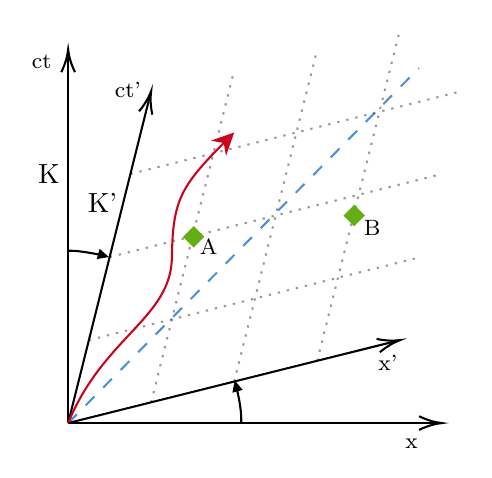
\begin{tikzpicture}[x=0.75pt,y=0.75pt,yscale=-1,xscale=1]
		
		%uncomment if require: \path (0,300); %set diagram left start at 0, and has height of 300
		
		%Straight Lines [id:da09228385528891703] 
		\draw    (50,250) -- (50,72) ;
		\draw [shift={(50,70)}, rotate = 90] [color={rgb, 255:red, 0; green, 0; blue, 0 }  ][line width=0.75]    (10.93,-3.29) .. controls (6.95,-1.4) and (3.31,-0.3) .. (0,0) .. controls (3.31,0.3) and (6.95,1.4) .. (10.93,3.29)   ;
		%Straight Lines [id:da4268461941251125] 
		\draw    (50,250) -- (228,250) ;
		\draw [shift={(230,250)}, rotate = 180] [color={rgb, 255:red, 0; green, 0; blue, 0 }  ][line width=0.75]    (10.93,-3.29) .. controls (6.95,-1.4) and (3.31,-0.3) .. (0,0) .. controls (3.31,0.3) and (6.95,1.4) .. (10.93,3.29)   ;
		%Straight Lines [id:da9487439459823469] 
		\draw [color={rgb, 255:red, 74; green, 144; blue, 226 }  ,draw opacity=1 ] [dash pattern={on 4.5pt off 4.5pt}]  (50,250) -- (219,79) ;
		%Straight Lines [id:da23686264430765613] 
		\draw    (50,250) -- (89.51,91.94) ;
		\draw [shift={(90,90)}, rotate = 104.04] [color={rgb, 255:red, 0; green, 0; blue, 0 }  ][line width=0.75]    (10.93,-3.29) .. controls (6.95,-1.4) and (3.31,-0.3) .. (0,0) .. controls (3.31,0.3) and (6.95,1.4) .. (10.93,3.29)   ;
		%Straight Lines [id:da2319306760067581] 
		\draw    (50,250) -- (208.06,210.49) ;
		\draw [shift={(210,210)}, rotate = 165.96] [color={rgb, 255:red, 0; green, 0; blue, 0 }  ][line width=0.75]    (10.93,-3.29) .. controls (6.95,-1.4) and (3.31,-0.3) .. (0,0) .. controls (3.31,0.3) and (6.95,1.4) .. (10.93,3.29)   ;
		%Straight Lines [id:da18195780417564067] 
		\draw [color={rgb, 255:red, 0; green, 0; blue, 0 }  ,draw opacity=0.4 ] [dash pattern={on 0.84pt off 2.51pt}]  (90,240) -- (130,80) ;
		%Straight Lines [id:da05857248799082826] 
		\draw [color={rgb, 255:red, 0; green, 0; blue, 0 }  ,draw opacity=0.4 ] [dash pattern={on 0.84pt off 2.51pt}]  (60,210) -- (220,170) ;
		%Straight Lines [id:da5221292993803834] 
		\draw [color={rgb, 255:red, 0; green, 0; blue, 0 }  ,draw opacity=0.4 ] [dash pattern={on 0.84pt off 2.51pt}]  (130,230) -- (170,70) ;
		%Straight Lines [id:da6761293595495029] 
		\draw [color={rgb, 255:red, 0; green, 0; blue, 0 }  ,draw opacity=0.4 ] [dash pattern={on 0.84pt off 2.51pt}]  (170,220) -- (210,60) ;
		%Straight Lines [id:da588553509786019] 
		\draw [color={rgb, 255:red, 0; green, 0; blue, 0 }  ,draw opacity=0.4 ] [dash pattern={on 0.84pt off 2.51pt}]  (70,170) -- (230,130) ;
		%Straight Lines [id:da25280593467601176] 
		\draw [color={rgb, 255:red, 0; green, 0; blue, 0 }  ,draw opacity=0.4 ] [dash pattern={on 0.84pt off 2.51pt}]  (80,130) -- (240,90) ;
		%Curve Lines [id:da8582723308387954] 
		\draw    (133.38,249.75) .. controls (133.6,245.13) and (132.65,239.15) .. (130.98,232.34) ;
		\draw [shift={(130.25,229.5)}, rotate = 75.12] [fill={rgb, 255:red, 0; green, 0; blue, 0 }  ][line width=0.08]  [draw opacity=0] (5.36,-2.57) -- (0,0) -- (5.36,2.57) -- cycle    ;
		%Curve Lines [id:da24906121093657063] 
		\draw    (50.13,167) .. controls (53.91,166.79) and (61.39,167.99) .. (66.8,169.27) ;
		\draw [shift={(69.63,170)}, rotate = 195.95] [fill={rgb, 255:red, 0; green, 0; blue, 0 }  ][line width=0.08]  [draw opacity=0] (5.36,-2.57) -- (0,0) -- (5.36,2.57) -- cycle    ;
		%Curve Lines [id:da53729283067976] 
		\draw [color={rgb, 255:red, 208; green, 2; blue, 27 }  ,draw opacity=1 ]   (50,250) .. controls (67.13,208.25) and (99.63,199.5) .. (100,170) .. controls (100.37,141.24) and (104.77,135.29) .. (128.16,111.84) ;
		\draw [shift={(130,110)}, rotate = 135] [fill={rgb, 255:red, 208; green, 2; blue, 27 }  ,fill opacity=1 ][line width=0.08]  [draw opacity=0] (10.72,-5.15) -- (0,0) -- (10.72,5.15) -- (7.12,0) -- cycle    ;
		%Shape: Diamond [id:dp3515169969756292] 
		\draw  [color={rgb, 255:red, 100; green, 173; blue, 18 }  ,draw opacity=1 ][line width=5]  (110.46,159.83) -- (110.92,160.29) -- (110.46,160.75) -- (110,160.29) -- cycle ;
		%Shape: Diamond [id:dp5984572223867858] 
		\draw  [color={rgb, 255:red, 100; green, 173; blue, 18 }  ,draw opacity=1 ][line width=5]  (187.79,149.58) -- (188.25,150.04) -- (187.79,150.5) -- (187.33,150.04) -- cycle ;
		
		% Text Node
		\draw (31,71) node [anchor=north west][inner sep=0.75pt]   [align=left] {{\footnotesize ct}};
		% Text Node
		\draw (34,124) node [anchor=north west][inner sep=0.75pt]   [align=left] {K};
		% Text Node
		\draw (211,256) node [anchor=north west][inner sep=0.75pt]   [align=left] {{\footnotesize x}};
		% Text Node
		\draw (198,216) node [anchor=north west][inner sep=0.75pt]   [align=left] {{\footnotesize x'}};
		% Text Node
		\draw (71,84) node [anchor=north west][inner sep=0.75pt]   [align=left] {{\footnotesize ct'}};
		% Text Node
		\draw (58,138) node [anchor=north west][inner sep=0.75pt]   [align=left] {K'};	
		% Text Node
		\draw (112,160) node [anchor=north west][inner sep=0.75pt]   [align=left] {{\footnotesize A}};	
		% Text Node
		\draw (191,151) node [anchor=north west][inner sep=0.75pt]   [align=left] {{\footnotesize B}};
	\end{tikzpicture}
	\caption{Un boost desde el sistema $K$ al $K'$, con las coordenadas del nuevo sistema superpuestas sobre las del antiguo. La línea de mundo de una partícula (en rojo) es invariable, pero sus coordenadas en cada sistema variarán. Además, dos eventos $A$ y $B$ pueden intercambiar orden temporal, si en el sistema $K$ ocurre $A$ y luego $B$, en el sistema $K'$ será al contrario. La línea azul corresponde a un objeto viajando a la velocidad de la luz. Ningún cuerpo podrá cruzar la línea azul (viajar más rápido que la luz), ya que las transformaciones de Lorentz son hiperbólicas.}
\end{figure}

Si bien un cambio de sistema puede cambiar el orden temporal de los eventos, no se puede cambiar la causalidad bajo ningún medio. Podemos representar el espacio de coordenadas que pueden afectar a un cierto evento con un \textit{cono de luz} proyectado al pasado, como se ve en la figura \ref{fig:cono_luz}.
\begin{figure}
	\centering
	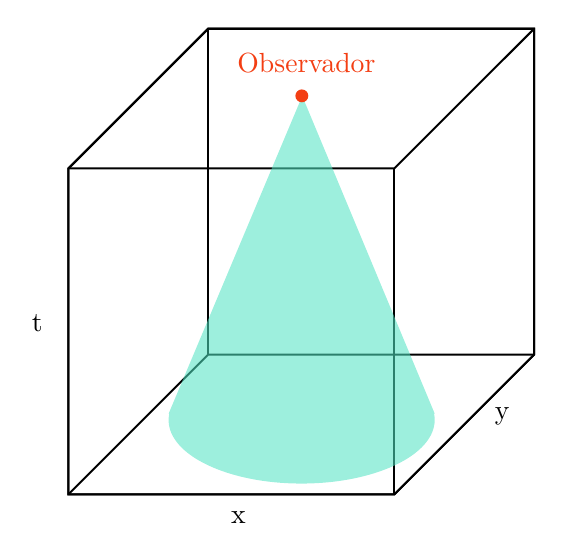
\begin{tikzpicture}[x=0.75pt,y=0.75pt,yscale=-1,xscale=1]

		%uncomment if require: \path (0,300); %set diagram left start at 0, and has height of 300
		
		%Shape: Cube [id:dp5286636250983902] 
		\draw  [line width=0.75]  (34.04,78.1) -- (101.34,10.8) -- (258.4,10.8) -- (258.4,167.84) -- (191.09,235.15) -- (34.04,235.15) -- cycle ; \draw  [line width=0.75]  (258.4,10.8) -- (191.09,78.1) -- (34.04,78.1) ; \draw  [line width=0.75]  (191.09,78.1) -- (191.09,235.15) ;
		%Shape: Cube [id:dp3761531917875258] 
		\draw  [line width=0.75]  (258.4,167.84) -- (191.09,235.15) -- (34.04,235.15) -- (34.04,78.1) -- (101.34,10.8) -- (258.4,10.8) -- cycle ; \draw  [line width=0.75]  (34.04,235.15) -- (101.34,167.84) -- (258.4,167.84) ; \draw  [line width=0.75]  (101.34,167.84) -- (101.34,10.8) ;
		
		%Shape: Path Data [id:dp6613974481621384] 
		\draw  [draw opacity=0][fill={rgb, 255:red, 80; green, 227; blue, 194 }  ,fill opacity=0.56 ] (210.53,196.27) -- (210.21,196.27) .. controls (210.42,197.28) and (210.52,198.3) .. (210.52,199.33) .. controls (210.46,216.24) and (181.71,229.94) .. (146.31,229.94) .. controls (110.91,229.94) and (82.26,216.24) .. (82.32,199.33) .. controls (82.32,198.3) and (82.43,197.28) .. (82.64,196.27) -- (82.33,196.27) -- (146.7,43.25) -- (209.12,192.9) .. controls (209.23,193.15) and (209.34,193.4) .. (209.44,193.65) -- (210.53,196.27) -- cycle ;
		%Shape: Ellipse [id:dp13935554349004498] 
		\draw  [draw opacity=0][fill={rgb, 255:red, 243; green, 62; blue, 19 }  ,fill opacity=1 ][line width=0.75]  (143.41,43.15) .. controls (143.41,41.44) and (144.8,40.05) .. (146.52,40.05) .. controls (148.23,40.05) and (149.62,41.44) .. (149.62,43.15) .. controls (149.62,44.87) and (148.23,46.26) .. (146.52,46.26) .. controls (144.8,46.26) and (143.41,44.87) .. (143.41,43.15) -- cycle ;
		
		% Text Node
		\draw (114,21) node [anchor=north west][inner sep=0.75pt]  [color={rgb, 255:red, 243; green, 62; blue, 19 }  ,opacity=1 ] [align=left] {Observador};
		% Text Node
		\draw (14.92,146.92) node [anchor=north west][inner sep=0.75pt]   [align=left] {t};
		% Text Node
		\draw (111,242) node [anchor=north west][inner sep=0.75pt]   [align=left] {x};
		% Text Node
		\draw (238,192) node [anchor=north west][inner sep=0.75pt]   [align=left] {y};
		
		
	\end{tikzpicture}
	\label{fig:cono_luz}
	\caption{Cono de luz de un cierto evento proyectado al pasado. Para que un evento pueda afectar al evento en rojo este debe ocurrir dentro del cono celeste, ya que, en cambio, si ocurre fuera de él deberá moverse a una velocidad más rápida que la luz.}
\end{figure}

La generalización de boosts de Lorentz a una velocidad arbitraria $\mathbf{v}$ se puede escribir como:
\begin{align}
	\mathbf{x}' &= \mathbf{x} + \mathbf{v}\left[\frac{\mathbf{x} \cdot \mathbf{v}}{v^2} \bar{\gamma} - \gamma t\right] \\
	t' &= \gamma \left(t - \frac{\mathbf{x} \cdot \mathbf{v}}{c^2}\right)
\end{align}
donde
\begin{align}
	\gamma &= \frac{1}{\sqrt{1 - v^2/c^2}}\\
	\bar{\gamma} &= \gamma - 1
\end{align}

O, en resumen, de forma compacta y matricial:
\begin{table}[h!]
	\centering
	\begin{tabular}{ccc}
		${A^\alpha}_\mu {A_\alpha}^\nu = {\delta^\nu}_\mu, \ \ $ & $\eta_{\alpha\beta} {\Lambda^\alpha}_\mu {\Lambda_\nu}^\beta = \eta_{\mu\nu},\ \ $ & ${\Lambda_\mu}^\alpha(\mathbf{v}) = [{\Lambda^{-1}(\mathbf{v})]^\alpha}_\mu \equiv {\Lambda^\alpha}_\mu(-\mathbf{v})$
	\end{tabular}
\end{table}

donde ${\Lambda^\mu}_\nu (\mathbf{v})$ es una matriz correspondiente al boost de Lorentz:
\begin{equation}
	\begin{pmatrix}
		\gamma & -v_x\gamma & -v_y\gamma & -v_z\gamma \\
		-\dfrac{v_x\gamma}{c^2} & 1+\dfrac{\bar{\gamma}v_x^2}{v^2} & \dfrac{\bar{\gamma}v_xv_y}{v^2} & \dfrac{\bar{\gamma}v_xv_z}{v^2}\\
		-\dfrac{v_y\gamma}{c^2} & \dfrac{\bar{\gamma}v_xv_y}{v^2} & 1+\dfrac{\bar{\gamma}v_y^2}{v^2} & \dfrac{\bar{\gamma}v_yv_z}{v^2}\\
		-\dfrac{v_z\gamma}{c^2} & \dfrac{\bar{\gamma}v_xv_z}{v^2} & \dfrac{\bar{\gamma}v_yv_z}{v^2} & 1+\dfrac{\bar{\gamma}v_z^2}{v^2} \\
	\end{pmatrix}
\end{equation}

Por ejemplo, un boost en la dirección $\mathbf{\hat{x}}$:
\begin{equation}
	{\Lambda^\mu}_\nu (v\mathbf{\hat{x}}) = \begin{pmatrix}
		\gamma & -v\gamma & 0 & 0 \\
		-v\gamma/c^2 & \gamma & 0 & 0\\
		0 & 0 & 1 & 0\\
		0 & 0 & 0 & 1 \\
	\end{pmatrix}
\end{equation}

\caja{Boost puro}{Se le dice boost puro a una transformación que no incluye rotaciones espaciales, es decir, que solo consiste en un salto de un marco estacionario a otro que se mueve a velocidad constante. La matriz ${\Lambda^\mu}_\nu$ para boosts puros es \textbf{siempre simétrica}.}

Si realizamos dos boosts consecutivos con velocidades $v_1$ y $v_2$ en la misma dirección $\mathbf{\hat{x}}$, la transformación combinada será un boost puro en dirección $\mathbf{\hat{x}}$ con rapidez (ángulo hiperbólico):
\begin{equation}
	\psi = \psi_1 + \psi_2 = \text{arctanh}\left(\frac{v_1}{c}\right) + \text{arctanh}\left(\frac{v_2}{c}\right) 
\end{equation}


Si, en cambio, realizamos dos boosts consecutivos con velocidades \(v_1\hat{x}\) y \(v_2\hat{y}\):
\begin{equation}
	\indUpDown[\Lambda_1] \equiv \LambdaMuNu(v_1\hat{x}),\ \ \ \indUpDown[\Lambda_2] \equiv \LambdaMuNu(v_2\hat{y}),
\end{equation}
la transformación final dependerá del orden en que aplicamos los boosts, es decir, los \textbf{boosts no son conmutativos} (\(\Lambda_1\cdot\Lambda_2\neq\Lambda_2\cdot\Lambda_1\)). Además, la transformación combinada ya no será un boost puro\footnote{Prueba: Tomando \(c=1\) y definiendo: \[\indUpDown[\Lambda_1] = \begin{pmatrix}
	\gamma(v_1) & -v_1\gamma(v_1) & 0 & 0\\
	-v_1\gamma(v_1) & \gamma(v_1) & 0 & 0\\
	0 & 0 & 1 & 0\\
	0 & 0 & 0 & 1
\end{pmatrix},\ \ \ \indUpDown[\Lambda_2] = \begin{pmatrix}
\gamma(v_2) & 0 & -v_2\gamma(v_2) & 0\\
0 & 1 & 0 & 0\\
-v_2\gamma(v_2) & 0 & \gamma(v_2) & 0\\
0 & 0 & 0 & 1
\end{pmatrix}\] Tendremos: \[\indUpDown[\Lambda_1][\mu][\alpha]\indUpDown[\Lambda_2][\alpha]= \begin{pmatrix}
\gamma(v_1)\gamma(v_2) & \textcolor{red}{-v_1\gamma(v_1)} & -v_2\gamma(v_2) & 0\\
\textcolor{blue}{-v_1\gamma(v_1)\gamma(v_2)} & \gamma(v_1) & \textcolor{magenta}{v_1v_2\gamma(v_1)\gamma(v_2)} & 0\\
-v_2\gamma(v_2) & \textcolor{olive}{0} & \gamma(v_2) & 0\\
0 & 0 & 0 & 1
\end{pmatrix}\]\[\indUpDown[\Lambda_2][\mu][\alpha]\indUpDown[\Lambda_1][\alpha]= \begin{pmatrix}
\gamma(v_1)\gamma(v_2) & \textcolor{red}{-v_1\gamma(v_1)\gamma(v_2)} & -v_2\gamma(v_2) & 0\\
\textcolor{blue}{-v_1\gamma(v_1)} & \gamma(v_1) & \textcolor{magenta}{0} & 0\\
-v_2\gamma(v_2) & \textcolor{olive}{v_1v_2\gamma(v_1)\gamma(v_2)} & \gamma(v_2) & 0\\
0 & 0 & 0 & 1
\end{pmatrix}\] Evidentemente, los valores coloreados son distintos, por lo que la multiplicación no es conmutativa y sus productos no son simétricos.}.

\subsection{Grupos de Lorentz}

\subsubsection{Grupos y álgebra de Lie crash course}
Hay dos tipos de grupos que nos interesan:
\begin{itemize}
	\item Especiales ortogonales de \(n\) dimensiones \((SO(n))\), cumplen con:
	\begin{equation}
		\det{\Lambda} = 1,\ \ \ \ \Lambda^T\Lambda = +1
	\end{equation}
	\item Especiales unitarias de \(n\) dimensiones \((SU(n))\), cumplen con:
	\begin{equation}
		\det{\Lambda} = 1,\ \ \ \ \Lambda^\dagger\Lambda = +1
	\end{equation}
\end{itemize}

\caja{Grupo de Lie (\(G\))}{Una variedad suave (i.e. infinitamente diferenciable) donde cada punto \(\Lambda\) es una transformación de simetría (i.e. deja \textit{alguna} propiedad invariable al transformar). Ejemplo: una esfera donde cada punto en su superficie representa una rotación en 3-D.}

Imagina que quieres hacer una transformación \(\Lambda\) que corresponda a una rotación de \(\theta\) grados. Usando una expansión de Taylor podemos reescribirlo como:
\begin{equation*}
	\Lambda(\theta)\approx I + X + \mathcal{O}(\theta^2)
\end{equation*}
Pero esto solo funciona cuando \(\theta\) es pequeño, si queremos expandirlo a cualquier rotación podemos \textit{componer} \(n\) rotaciones pequeñas:
\begin{equation*}
	\Lambda(\theta)\approx \left(I + \frac{\theta}{n}X\right)\left(I + \frac{\theta}{n}X\right)\cdots = \left(I + \frac{\theta}{n}X\right)^n
\end{equation*}
Y, finalmente, tendremos una equivalencia exacta cuando tomamos \(n\) infinitos y pasos infinitesimales:
\begin{equation}
	\Lambda(\theta) = \lim_{n\rightarrow\infty}\left(I + \frac{\theta}{n}X(\frac{\theta}{n})\right)^n = e^{\theta X}
	\label{eqn:map_gem_trans}
\end{equation}

\caja{Álgebra de Lie (\(\mathfrak{g}\))}{Espacio vectorial tangente a \(G\) en la identidad \(I\).}

Si bien un álgebra de Lie es una aproximación del grupo en un punto, podemos recuperar cualquier transformación\footnote{Siempre y cuando esté conectada desde la identidad! Un flip de espejo no se puede recrear.} que vive en el grupo a partir de pasitos infinitesimales definidos por el álgebra.

Una álgebra de Lie es un espacio vectorial, por lo que toda transformación infinitesimal puede ser escrita como una combinación linear de bases llamadas \textbf{generadores}.

Como cualquier grupo, \(\mathfrak{g}\) debe cumplir con las propiedades de un grupo, llámese:
\begin{enumerate}
	\item Clausura con respecto a la multiplicación: toma dos transformaciones infinitesimales y el producto de aplicar ambas es también una transformación del álgebra.
	\item Asociatividad: \((A\cdot B)\cdot C = A\cdot(B\cdot C) \).
	\item Elemento unitario: \(I\).
	\item Elemento inverso.
\end{enumerate}
Nótese que estos requerimientos no incluyen conmutatividad (\(A\cdot B \neq B\cdot A\)).

\caja{Conmutador}{Sabemos que una combinación lineal de elementos debe ser también elemento del grupo, pero el orden de aplicación importa para el resultado final. Podemos "cuantificar el fracaso" al conmutar  definiendo una operación: \[[X, Y] = XY - YX\] Es decir, la diferencia al cambiar el orden entre dos operaciones. Tendremos que \([X,Y] = -[Y,X]\)}

En general, tendremos la relación:
\begin{equation}
	[T_a,T_b]=f_{abc}T_c,
\end{equation}
donde \(T_a,T_b,T_c\) son vectores o elementos del grupo del álgebra, y \(f_{abc}\) es una \textbf{constante de estructura}.

Como tenemos que una matriz \(R\) de \(SO(n)\) cumple con \(R^T R = 1\) y \(R \approx I + \epsilon A\), donde \(A\) es un generador. Si juntamos ambas ecuaciones llegamos a:
\begin{align*}
	(I + \epsilon A)^T (I + \epsilon A) &= I\\
	I + \epsilon(A + A^T) + \mathcal{O}(\epsilon^2) &= I
\end{align*}
\begin{equation}
	\Rightarrow A^T = -A
\end{equation}
por lo que los generadores \(A\) son \textbf{matrices antisimétricas}. Con un proceso idéntico también llegamos a que las matrices generadoras de \(SU(n)\) son \textbf{anti-hermitianas} (\(X^\dagger=-X\)) y \textbf{sin traza} (\(\text{Tr}(X)=0\)).

\subsubsection{Álgebra de grupos de Lorentz}
Si \(\LambdaMuNu\) son las transformaciones de Lorentz posibles en 3+1 dimensiones (\(SO(1,3)\)), tendremos un grupo de Lie definido por 6 bases (\(\mathfrak{so}(1,3)\)):
\begin{itemize}
	\item 3 rotaciones espaciales (en los planos \(xy, yz, xz\)):
	\begin{equation}
		\indUpDown[J][a][bc] = -i \epsilon_{abc}
	\end{equation}
	\item 3 boosts de Lorentz (rotaciones en los planos \(xt, yt, zt\)):
	\begin{equation}
		\indUpDown[K][a\mu][\ \nu] = i(\indUpDown[\delta][\mu][a]\delta_{\nu 0} + \indUpDown[\delta][\mu][0]\delta_{\nu a})
	\end{equation}
\end{itemize}

Los generadores de los boosts y rotaciones serán entonces, respectivamente:
\begin{equation}
	\begin{matrix}
		K^x = \begin{pmatrix}
			\0 &i &\0 &\0\\
			i &\0 &\0 &\0\\
			\0 &\0 &\0 &\0\\
			\0 &\0 &\0 &\0
		\end{pmatrix} & 
		K^y = \begin{pmatrix}
		\0 &\0 &i &\0\\
		\0 &\0 &\0 &\0\\
		i &\0 &\0 &\0\\
		\0 &\0 &\0 &\0
		\end{pmatrix} &
		K^z = \begin{pmatrix}
		\0 &\0 &\0 &i\\
		\0 &\0 &\0 &\0\\
		\0 &\0 &\0 &\0\\
		i &\0 &\0 &\0
		\end{pmatrix}
	\end{matrix}
\end{equation}
\begin{equation}
	\begin{matrix}
		J^x = \begin{pmatrix}
			\0 &\0 &\0 &\0\\
			\0 &\0 &\0 &\0\\
			\0 &\0 &\0 &-i\\
			\0 &\0 &i &\0
		\end{pmatrix} & 
		J^y = \begin{pmatrix}
			\0 &\0 &\0 &\0\\
			\0 &\0 &\0 &i\\
			\0 &\0 &\0 &\0\\
			\0 &-i &\0 &\0
		\end{pmatrix} &
		J^z = \begin{pmatrix}
			\0 &\0 &\0 &\0\\
			\0 &\0 &-i &\0\\
			\0 &i &\0 &\0\\
			\0 &\0 &\0 &\0
		\end{pmatrix}
	\end{matrix}
\end{equation}
(recuerda: estas matrices no definen transformaciones, sino que bloques para construirlas. Las transformaciones tendrán una matriz identidad sumada como mínimo).

Las constantes de estructura dependerán de las diferentes combinaciones de bases, tendremos que:
\begin{equation}
	\begin{matrix}
		[K^a,K^b] = -i\epsilon_{abc}J^c,\ \ \ \ & [K^a,J^b] = i\epsilon_{abc}K^c,\ \ \ \ & [J^a,J^b] = i\epsilon_{abc}J^c
	\end{matrix}
\end{equation}

Los boosts sin rotaciones no forman una subálgebra, pero las rotaciones por sí solas \textbf{forman una subálgebra} (\(\mathfrak{so}(3)\)).

Peeero, si definimos los generadores:
\begin{equation}
	T^{(\pm)}_a = \frac{(J_a \pm iK_a)}{2}
\end{equation}
Podemos definir dos subálgebras \(\left\lbrace T^{(+)}_a,T^{(-)}_a\right\rbrace\) que sí son cerradas y conmutan entre sí:
\begin{equation}
	\begin{matrix}
		[T^{(+)}_a,T^{(+)}_b] = i\epsilon_{abc}T^{(+)}_c,\ \ \ \ & [T^{(-)}_a,T^{(-)}_b] = i\epsilon_{abc}T^{(-)}_c,\ \ \ \ & [T^{(+)}_a,T^{(-)}_b] = 0
	\end{matrix}
\end{equation}
donde cada subálgebra será \(\mathfrak{so}(3)\), por lo que podemos escribir \(\mathfrak{so}(1,3)_\mathbb{C}\cong\mathfrak{so}(3)\oplus\mathfrak{so}(3)\), es decir, el álgebra completa se puede subdividir en dos piezas que no interactúan entre sí. Además, como estamos usando valores  complejos, salo fácilmente que \(\mathfrak{so}(3)\oplus\mathfrak{so}(3) \sim \mathfrak{su}(2)\oplus\mathfrak{su}(2)\)\footnote{\(\mathfrak{so}(3)\) son matrices reales antisimétricas en 3-D, por lo que tienen 3 variables independientes:
\[\begin{pmatrix}
	0 & a & b\\
	-a & 0 & c\\
	-b & -c & 0
\end{pmatrix},\]mientras que \(\mathfrak{su}(2)\) son matrices complejas hermíticas sin traza en 2-D, por lo que también tienen 3 variables independientes:
\[\begin{pmatrix}
a & b+ic\\
b-ic & -a
\end{pmatrix}\]}.

Para pasar de generadores a transformaciones explícitas, recordamos la ecuación \ref{eqn:map_gem_trans} para obtener:
\begin{equation}
	\mathcal{T}_a^\pm (\theta\hat{\theta}) = e^{i\theta(J_a \pm iK_a)}
\end{equation}

\subsubsection{Espacios de representación y operador Casimir (\(\mathcal{\hat{C}}\)}
A partir de nuestro espacio de Minkowski podemos mapear cada punto a un elemento específico. Por ejemplo, podemos tener un espacio escalar que asigne un número que represente temperatura a cada punto del espacio-tiempo. O un espacio \(\mathbb{R}^{(1,3)}\) que asigne un vector 4-D que represente la posición espacio-temporal a cada punto, esencialmente lo que llevamos haciendo desde el principio. Puede hacerse lo mismo con otras construcciones: tensores, spinors, etc. Estos espacios se llaman \textbf{espacios de representación}.

\caja{Casimir (\(\mathcal{\hat{C}}\))}{Un operador Casimir (\(\mathcal{\hat{C}}\)) es aquel que conmuta con todos los generadores \begin{equation}
		[T_a,\mathcal{\hat{C}}] = 0
\end{equation}
Cada representación irreducible (los bloques fundamentales del grupo, las subalgebras que no pueden subdividirse más) es completamente caracterizada por un valor propio de Casimires. Cantidad de Casimires = rango del grupo.}

Al aplicar un Casimir sobre un objeto de una cierta representación obtendremos siempre el mismo resultado, por lo que podemos usar tal valor para etiquetar las diferentes representaciones.

En el caso del álgebra de Lorentz  \(\sim\mathfrak{so}(3)\oplus\mathfrak{so}(3)\), por lo que esperamos dos Casimires:
\begin{equation}
	\mathcal{\hat{C}}_{\pm} = \sum_{a}(T_a^{\pm})^2 = \frac{\mathbf{J}^2-\mathbf{K}^2}{4} \pm i\frac{\mathbf{J}\cdot\mathbf{K}}{2}
\end{equation}
El rango de un grupo de Lorentz es 2; cada representación irreducible del álgebra de Lorentz es caracterizada por valores propios de dos Casimires.

En el caso del espacio de representación de Minkowski, tendremos que ambos Casimires serán:
\begin{equation}
	\mathcal{\hat{C}}_{\pm} = \frac{3}{4}\mathbb{I}
\end{equation}
Es decir, aplicar un Casimir sobre cualquier vector 4-D obtendremos el mismo vector multiplicado por \(3/4\). Por ende, usaremos las etiquetas \((3/4,3/4)\) para etiquetar la representación de vectores 4-D.

\subsection{Consecuencias físicas}
\subsubsection{Intervalos}
Para un boost \(v\) en una dirección arbitraria, y recordando que:
\begin{equation*}
	\gamma(v) \equiv \frac{1}{1-v^2/c^2}
\end{equation*}
Tendremos que los intervalos de tiempo y espacio en dirección longitudinal cambiarán entre el marco estático (el laboratorio) y marco en movimiento (el punto de vista del objeto), y serán, respectivamente:
\begin{align}
	\Delta t_{\text{lab}} = \gamma(v)\Delta t_{\text{r.f.}}\\
	\Delta L_{\text{lab}} = \frac{\Delta L_{\text{r.f.}}}{\gamma(v)}
\end{align}
mientras que las distancias transversales no cambiarán.

\begin{figure}
	\centering	
	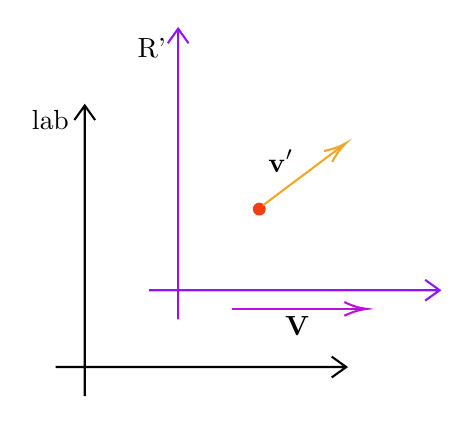
\begin{tikzpicture}[x=0.75pt,y=0.75pt,yscale=-1,xscale=1]
		%uncomment if require: \path (0,300); %set diagram left start at 0, and has height of 300
		
		%Shape: Axis 2D [id:dp09183262576503148] 
		\draw  (15,186) -- (155,186)(29,60) -- (29,200) (148,181) -- (155,186) -- (148,191) (24,67) -- (29,60) -- (34,67)  ;
		%Shape: Axis 2D [id:dp613381092730583] 
		\draw [color={rgb, 255:red, 144; green, 19; blue, 254 }  ,draw opacity=1 ] (60,149) -- (200,149)(74,23) -- (74,163) (193,144) -- (200,149) -- (193,154) (69,30) -- (74,23) -- (79,30)  ;
		%Shape: Ellipse [id:dp35952328928937094] 
		\draw  [draw opacity=0][fill={rgb, 255:red, 243; green, 62; blue, 19 }  ,fill opacity=1 ][line width=0.75]  (110,109.9) .. controls (110,108.18) and (111.39,106.79) .. (113.1,106.79) .. controls (114.82,106.79) and (116.21,108.18) .. (116.21,109.9) .. controls (116.21,111.61) and (114.82,113) .. (113.1,113) .. controls (111.39,113) and (110,111.61) .. (110,109.9) -- cycle ;
		%Straight Lines [id:da6086703750316328] 
		\draw [color={rgb, 255:red, 245; green, 166; blue, 35 }  ,draw opacity=1 ]   (115,108) -- (153.4,79.2) ;
		\draw [shift={(155,78)}, rotate = 143.13] [color={rgb, 255:red, 245; green, 166; blue, 35 }  ,draw opacity=1 ][line width=0.75]    (10.93,-3.29) .. controls (6.95,-1.4) and (3.31,-0.3) .. (0,0) .. controls (3.31,0.3) and (6.95,1.4) .. (10.93,3.29)   ;
		%Straight Lines [id:da36574170383458837] 
		\draw [color={rgb, 255:red, 189; green, 16; blue, 224 }  ,draw opacity=1 ]   (100,158) -- (163,158) ;
		\draw [shift={(165,158)}, rotate = 180] [color={rgb, 255:red, 189; green, 16; blue, 224 }  ,draw opacity=1 ][line width=0.75]    (10.93,-3.29) .. controls (6.95,-1.4) and (3.31,-0.3) .. (0,0) .. controls (3.31,0.3) and (6.95,1.4) .. (10.93,3.29)   ;
		
		% Text Node
		\draw (116,80) node [anchor=north west][inner sep=0.75pt]   [align=left] {$\displaystyle \mathbf{v} '$};
		% Text Node
		\draw (124,160) node [anchor=north west][inner sep=0.75pt]   [align=left] {$\displaystyle \mathbf{V}$};
		% Text Node
		\draw (2,61) node [anchor=north west][inner sep=0.75pt]   [align=left] {lab};
		% Text Node
		\draw (53,26) node [anchor=north west][inner sep=0.75pt]   [align=left] {R'};
	\end{tikzpicture}
\end{figure}
Si tenemos una partícula que se mueve con velocidad \(v'\) en un sistema de referencia \(R'\), que asu vez se mueve en dirección \(\hat{x}\) en el sistema del laboratorio con velocidad constante \(V\). Tendremos que, cuando las velocidades son arbitrarias, las transformaciones serán:
\begin{equation}
	\begin{matrix}
		\mathbf{x} = \mathbf{x}' + \mathbf{V}\left[\dfrac{\mathbf{x}'\cdot\mathbf{V}}{V^2}(\gamma-1) + \gamma t'\right],& t=\gamma\left(t' + \dfrac{\mathbf{x}'\cdot\mathbf{V}}{c^2}\right), & \gamma = \dfrac{1}{1-V^2/c^2}
	\end{matrix}
\end{equation}
\begin{equation}
	\mathbf{v} = \dfrac{d\mathbf{x}}{dt} = \dfrac{\mathbf{v}' + \mathbf{V}\left[\frac{\mathbf{v}'\cdot\mathbf{V}}{V^2}(\gamma-1) + \gamma \right] }{\gamma\left(1 + \frac{\mathbf{v}'\cdot\mathbf{V}}{c^2}\right)}
\end{equation}
\begin{align}
	v_x =\dfrac{dx}{dt} &= \dfrac{dx' + Vdt'}{dt' + \frac{Vdx'}{c^2}} = \dfrac{v_x' + V}{1 + \frac{v_x' V}{c^2}}\\
	v_y =\dfrac{dy}{dt} &= \dfrac{dy'}{\gamma\left( dt' + \frac{Vdx'}{c^2}\right)} = \dfrac{v_y'}{\gamma\left( dt' + \frac{Vdx'}{c^2}\right)}
\end{align}
La transformación de velocidad tiene términos no lineares, por lo que es complicada para utilizar (más que nada por la transformación del denominador temporal \(dt\rightarrow dt'\)).

\subsection{Formulación covariante}
Queremos formular todas las ecuaciones con cantidades covariantes, de forma que la estructura general se mantenga sin importar la transformación. La formulación clásica es covariante frente a transformaciones como rotaciones en el espacio 3-D, pero, al incluir boosts de Lorentz, la covarianza se pierde.

Por ello cambiaremos algunos de los objetos matemáticos que usamos:
\begin{itemize}
	\item El símbolo de Levi-Civita en 3 dimensiones no es Lorentz-covariante, se debe cambiar por su versión en 4 dimensiones (pero funciona igual).
	\begin{equation}
		\epsilon_{abc} \rightarrow \epsilon_{\mu\nu\alpha\beta}
	\end{equation}
	\item Los vectores:
	\begin{equation}
		\vec{a} \rightarrow a^\mu, a_\mu = \eta_{\mu\nu}a^\nu
	\end{equation}
	\item El producto escalar:
	\begin{equation}
		\vec{a}\cdot\vec{b} \rightarrow a_\mu b^\mu \equiv \eta_{\mu\nu}a^\mu b^\nu
	\end{equation}
	\item En vez de productos cruz (solo definido en 3-D):
	\begin{equation*}
		\vec{A}\times\vec{B} = (A_j B_k - A_k B_j)\hat{i} + (A_k B_i - A_i B_k)\hat{j} + (A_i B_j - A_j B_i)\hat{k}
	\end{equation*}
	tendremos un \textit{bivector}, un tensor antisimétrico de rango 2 :
	\begin{equation}
		A\wedge B = \frac{1}{2}(A^\mu B^\nu - A^\nu B^\mu)
	\end{equation}
	\item El gradiente:
	\begin{equation}
		\vec{\nabla} f \rightarrow \partial_\mu f
	\end{equation}
	\item La divergencia:
	\begin{equation}
		\nabla\cdot\vec{a} \equiv \partial_k a^k \rightarrow \partial_\mu f^\mu \equiv \eta^{\mu\nu}\partial_\mu f_\nu
	\end{equation}
	\item El rotacional:
	\begin{equation}
		\vec{\nabla}\times\vec{a} \rightarrow \partial_\mu a_\nu - \partial_\nu a_\mu
	\end{equation}
	\item El laplaciano:
	\begin{equation}
		\Delta \equiv \nabla^2 \equiv \partial_k^2 \rightarrow \square \equiv \partial_\mu\partial^\mu = \frac{\partial_t^2}{c^2} - \Delta
	\end{equation}
	\item En vez de un elemento de superficie:
	\begin{align*}
	d\vec{S} = d\vec{a} \times d\vec{b} &= (da_j db_k - da_k db_j)\hat{i} + (da_k db_i - da_i db_k)\hat{j} + (da_i db_j - da_j db_i)\hat{k}\\
	&= \hat{n}\left|dS\right| 
	\end{align*}
	tendremos el elemento de superficie (una 2-forma, bivector):
	\begin{equation}
	dS^{\mu\nu} = da^\mu db^\nu - db^\mu da^\nu
	\end{equation}
\end{itemize}

\subsubsection{4-velocidad propia}
Definiendo el intervalo de \textbf{tiempo propio} medido en el marco de referencia de la partícula:
\begin{equation}
	d\tau = \sqrt{1-v^2/c^2}dt
\end{equation}
Definimos la \textbf{4-velocidad propia}:
\begin{align}
	u^\mu \equiv \frac{dx^mu}{d\tau} &= \left(\dfrac{c}{\sqrt{1 - v^2/c^2}}, \dfrac{\vec{v}}{\sqrt{1 - v^2/c^2}} \right) \\
	u^\mu &= \left(\gamma c, \gamma\vec{v} \right)
\end{align}
La norma del vector 4-velocidad cumple con:
\begin{equation}
	u_\mu u^\mu \equiv \eta_{\mu\nu}u^\mu u^\nu = c^2
\end{equation}
Si conocemos todas las componentes de la 4-velocidad, podemos recuperar la velocidad normal sin conocer directamente el valor \(\gamma\) a través de:
\begin{equation}
	v^i = c\frac{u^i}{u^0}
\end{equation}

Vale recalcar que, a menos que trabajemos en el sistema propio del cuerpo, estaremos mezclando coordenadas de dos marcos de referencia distintos (la parte espacial será de un sistema arbitrario y el temporal del sistema propio). Por ello, no comparar con velocidad normal, podemos tener velocidades propias mayores que la \(c\).

\subsubsection{4-momento propio}
Siguiendo la misma idea, definimos el 4-momento covariante como:
\begin{equation}
	p^\mu \equiv mu^\mu = \left(\dfrac{mc}{\sqrt{1 - v^2/c^2}}, \dfrac{m\vec{v}}{\sqrt{1 - v^2/c^2}} \right) 
\end{equation}
De donde identificamos los componentes:
\begin{equation}
	\begin{matrix}
		p^\mu  = \left(\dfrac{E}{c}, \vec{p}\right), & E = \gamma mc^2, & \vec{p} = \gamma m\vec{v}
	\end{matrix}
\end{equation}
Consecuencia: una partícula tiene una energía en reposo enorme: \(E_{\text{rest}}=mc^2\). Además, de aquí obtenemos que\footnote{Prueba: \(p^\mu p_\mu = \dfrac{E^2}{c^2} - \vec{p}^{\ 2} \Rightarrow m^2u^2 = \dfrac{E^2}{c^2} - \vec{p}^{\ 2}\), pero \(u^2 = c^2\), por lo que \(m^2c^2 = \dfrac{E^2}{c^2} - \vec{p}^{\ 2} \Rightarrow m^2c^4 = E^2 - \vec{p}^{\ 2}c^2 \).}:
\begin{align}
	E^2 - \vec{p}^{\ 2}c^2 &= m^2c^4 \label{eqn:relacion_energia_momento}\\
	\Rightarrow E &= \sqrt{m^2c^4 + \sum p_i^2c^2}
\end{align}
(intentaré ser consistente al usar \(\vec{p}\) o \(p_i\) como 3-momento y \(p^\mu\) como 4-momento).

Por construcción, los componentes del 4-vector \(p^\mu\) transforman como coordenadas \(x^\mu\) o 4-velocidad \(u^\mu\):
\begin{equation}
	p'^\mu = \LambdaMuNu p^\nu
\end{equation}

Para un sistema de \(n\) partículas usaremos la notación:
\begin{equation}
	P^\mu = \sum_i^n p^\mu_i
\end{equation}

\subsubsection{4-fuerza}
Para la 4-fuerza definiremos:
\begin{equation}
	g^\mu \equiv \frac{dp^\mu}{d\tau} = \left(\dfrac{\vec{f}\cdot\vec{v}}{c\sqrt{1 - v^2/c^2}}, \dfrac{\vec{f}}{\sqrt{1 - v^2/c^2}} \right) 
\end{equation}
donde \(\vec{f}\) es la 3-fuerza \(\vec{f}=d\vec{p}/dt\).

Además se cumplirá que\footnote{Prueba: \(u_\mu u^\mu = \eta_{\mu\nu}u^\mu u^\nu = c^2 \Rightarrow \dfrac{d}{d\tau}(\eta_{\mu\nu}u^\mu u^\nu) = \dfrac{d}{d\tau}(c^2) \Rightarrow \eta_{\mu\nu}\dfrac{du^\mu}{d\tau}u^\nu + \eta_{\mu\nu}u^\mu\dfrac{du^\nu}{d\tau} = 0\). Pero en la primera parte de la primera mitad podemos hacer \(\mu\rightarrow\nu\), pero por simetría \(\eta_{\mu\nu}=\eta_{\nu\mu}\), por lo que: \(\eta_{\mu\nu}\dfrac{du^\nu}{d\tau}u^\mu + \eta_{\mu\nu}u^\mu\dfrac{du^\nu}{d\tau} = 0 \Rightarrow 2\eta_{\mu\nu}u^\mu\dfrac{du^\nu}{d\tau} = 0 \Rightarrow 2\eta_{\mu\nu}u^\mu\dfrac{1}{m}\dfrac{dp^\nu}{d\tau} = 0 \Rightarrow \dfrac{2}{m} u^\mu \eta_{\mu\nu} g^\nu = 0 \Rightarrow u^\mu g_\mu = 0\).}:
\begin{equation}
	u^\mu g_\mu = 0
\end{equation}

\subsection{Colisiones}
Algunas cosas a tener cuidado:
\begin{itemize}
	\item No se permiten interacciones a distancia, términos como \(U(\vec{r}_1 - \vec{r}_2)\) no pueden aparecer en la acción.
	\item Los \textit{campos} llevan parte de la energía-momento del sistema.
	\item Se pierde la noción de \textit{centro de masa}, ya que distintos observadores verán partículas  moviéndose distinto unas de otras. Pero podemos definir un marco \(C\) que cumpla con que el 3-momento neto sea nulo:
	\begin{equation*}
		\sum \vec{p}_i = 0
	\end{equation*}
\end{itemize}

\subsubsection{Conservación de Energía-Momento}
El teorema de Noether nos dice que si tenemos un sistema de \(n\) partículas, entonces tenemos conservación de energía-momento. En notación covariante diríamos:
\begin{equation}
	P^\mu = \text{const.}
\end{equation}
O, de otra manera:
\begin{equation}
	P^\mu_{\text{inicial}} = P^\mu_{\text{final}} \label{eqn:cons_energia_momento}
\end{equation}
Las masas individuales de las partículas pueden cambiar antes y después de un evento (como una desintegración), pero la \textbf{masa invariante} (\(M\)) del sistema se debe mantener constante:
\begin{equation}
	P^\mu P_\mu = M^2c^2
\end{equation}

\subsubsection{Scattering elástico relativista}
Llamaremos colisión o scattering elástico a cualquier interacción que tenga la misma cantidad de partículas antes y después de esta, y que conserve la masa en reposo de cada partícula.
\begin{figure}[h]
	\centering
	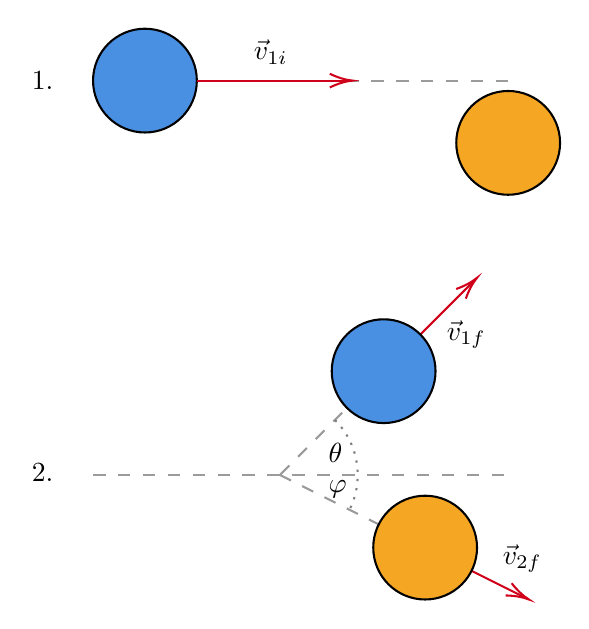
\begin{tikzpicture}[x=0.75pt,y=0.75pt,yscale=-1,xscale=1]
		%uncomment if require: \path (0,300); %set diagram left start at 0, and has height of 300
		
		%Straight Lines [id:da2537740026274753] 
		\draw [color={rgb, 255:red, 155; green, 155; blue, 155 }  ,draw opacity=1 ] [dash pattern={on 4.5pt off 4.5pt}]  (95,35) -- (245,35) ;
		%Shape: Circle [id:dp18483932320052876] 
		\draw  [fill={rgb, 255:red, 74; green, 144; blue, 226 }  ,fill opacity=1 ] (45,35) .. controls (45,21.19) and (56.19,10) .. (70,10) .. controls (83.81,10) and (95,21.19) .. (95,35) .. controls (95,48.81) and (83.81,60) .. (70,60) .. controls (56.19,60) and (45,48.81) .. (45,35) -- cycle ;
		%Shape: Circle [id:dp583423662308532] 
		\draw  [fill={rgb, 255:red, 245; green, 166; blue, 35 }  ,fill opacity=1 ] (220,65) .. controls (220,51.19) and (231.19,40) .. (245,40) .. controls (258.81,40) and (270,51.19) .. (270,65) .. controls (270,78.81) and (258.81,90) .. (245,90) .. controls (231.19,90) and (220,78.81) .. (220,65) -- cycle ;
		%Straight Lines [id:da9184970738123618] 
		\draw [color={rgb, 255:red, 208; green, 2; blue, 27 }  ,draw opacity=1 ]   (95,35) -- (168,35) ;
		\draw [shift={(170,35)}, rotate = 180] [color={rgb, 255:red, 208; green, 2; blue, 27 }  ,draw opacity=1 ][line width=0.75]    (10.93,-3.29) .. controls (6.95,-1.4) and (3.31,-0.3) .. (0,0) .. controls (3.31,0.3) and (6.95,1.4) .. (10.93,3.29)   ;
		%Straight Lines [id:da8462520792924382] 
		\draw [color={rgb, 255:red, 155; green, 155; blue, 155 }  ,draw opacity=1 ] [dash pattern={on 4.5pt off 4.5pt}]  (45,225) -- (245,225) ;
		%Straight Lines [id:da12868147120554208] 
		\draw [color={rgb, 255:red, 208; green, 2; blue, 27 }  ,draw opacity=1 ]   (200,160) -- (228.59,131.41) ;
		\draw [shift={(230,130)}, rotate = 135] [color={rgb, 255:red, 208; green, 2; blue, 27 }  ,draw opacity=1 ][line width=0.75]    (10.93,-3.29) .. controls (6.95,-1.4) and (3.31,-0.3) .. (0,0) .. controls (3.31,0.3) and (6.95,1.4) .. (10.93,3.29)   ;
		%Straight Lines [id:da42553824213503266] 
		\draw [color={rgb, 255:red, 155; green, 155; blue, 155 }  ,draw opacity=1 ] [dash pattern={on 4.5pt off 4.5pt}]  (165,195) -- (135,225) ;
		%Shape: Circle [id:dp0012112820079067665] 
		\draw  [fill={rgb, 255:red, 74; green, 144; blue, 226 }  ,fill opacity=1 ] (160,175) .. controls (160,161.19) and (171.19,150) .. (185,150) .. controls (198.81,150) and (210,161.19) .. (210,175) .. controls (210,188.81) and (198.81,200) .. (185,200) .. controls (171.19,200) and (160,188.81) .. (160,175) -- cycle ;
		%Straight Lines [id:da4205479401379062] 
		\draw [color={rgb, 255:red, 155; green, 155; blue, 155 }  ,draw opacity=1 ] [dash pattern={on 4.5pt off 4.5pt}]  (135,225) -- (195,255) ;
		%Straight Lines [id:da5920176859850526] 
		\draw [color={rgb, 255:red, 208; green, 2; blue, 27 }  ,draw opacity=1 ]   (195,255) -- (253.21,284.11) ;
		\draw [shift={(255,285)}, rotate = 206.57] [color={rgb, 255:red, 208; green, 2; blue, 27 }  ,draw opacity=1 ][line width=0.75]    (10.93,-3.29) .. controls (6.95,-1.4) and (3.31,-0.3) .. (0,0) .. controls (3.31,0.3) and (6.95,1.4) .. (10.93,3.29)   ;
		%Shape: Circle [id:dp11045125337722494] 
		\draw  [fill={rgb, 255:red, 245; green, 166; blue, 35 }  ,fill opacity=1 ] (180,260) .. controls (180,246.19) and (191.19,235) .. (205,235) .. controls (218.81,235) and (230,246.19) .. (230,260) .. controls (230,273.81) and (218.81,285) .. (205,285) .. controls (191.19,285) and (180,273.81) .. (180,260) -- cycle ;
		%Shape: Arc [id:dp29030415058117676] 
		\draw  [draw opacity=0][dash pattern={on 0.84pt off 2.51pt}] (161.57,198.53) .. controls (168.32,205.32) and (172.5,214.67) .. (172.5,225) .. controls (172.5,231.03) and (171.08,236.73) .. (168.55,241.78) -- (135,225) -- cycle ; \draw  [color={rgb, 255:red, 128; green, 128; blue, 128 }  ,draw opacity=1 ][dash pattern={on 0.84pt off 2.51pt}] (161.57,198.53) .. controls (168.32,205.32) and (172.5,214.67) .. (172.5,225) .. controls (172.5,231.03) and (171.08,236.73) .. (168.55,241.78) ;  
		
		% Text Node
		\draw (121,14) node [anchor=north west][inner sep=0.75pt]   [align=left] {$\displaystyle \vec{v}_{1i}$};
		% Text Node
		\draw (214,149) node [anchor=north west][inner sep=0.75pt]   [align=left] {$\displaystyle \vec{v}_{1f}$};
		% Text Node
		\draw (241,257) node [anchor=north west][inner sep=0.75pt]   [align=left] {$\displaystyle \vec{v}_{2f}$};
		% Text Node
		\draw (157,208) node [anchor=north west][inner sep=0.75pt]   [align=left] {$\displaystyle \theta $};
		% Text Node
		\draw (157,226) node [anchor=north west][inner sep=0.75pt]   [align=left] {$\displaystyle \varphi $};
		% Text Node
		\draw (14,29) node [anchor=north west][inner sep=0.75pt]   [align=left] {1.};
		% Text Node
		\draw (14,218) node [anchor=north west][inner sep=0.75pt]   [align=left] {2.};
	\end{tikzpicture}
\end{figure}

Para una colisión \(1+2\rightarrow 3+4\) tenemos 16 variables para definir todo el sistema, ya que tendremos 4 partículas con 4 componentes de 4-momento (energía, \(p_x,p_y,p_z\)). Sin embargo, podemos definir una serie de ecuaciones que restringirán al sistema y reducirán el número de partículas:
\begin{itemize}
	\item De la ecuación \ref{eqn:relacion_energia_momento} tenemos la condición de masa \textit{on shell} que nos da una ecuación para cada partícula (\textbf{4 en total}):
	\begin{equation*}
		E_i^2 - \vec{p}_i^{\ 2}c^2 = m_i^2c^4
	\end{equation*}
	\item De la conservación de 4-momento en la expresión \ref{eqn:cons_energia_momento} sacamos una ecuación por componente (\textbf{4 en total}):
	\begin{equation*}
		P^\mu_{\text{inicial}} = P^\mu_{\text{final}}
	\end{equation*}
	\item Podemos exigir que una de las partículas se mantenga en reposo al momento de la colisión, lo que nos daría expresiones para anular los componentes espaciales de su momento (\textbf{3 en total}).
	\begin{equation*}
		\vec{p}_2 = \vec{0}
	\end{equation*}
	\item También podemos hacer una rotación espacial para hacer coincidir la dirección del momento con el eje \(z\), dándonos 2 expresiones para anular las otras componentes del momento espacial (\textbf{2 en total}):
	\begin{equation*}
		p_{1x} = 0,\ \ \ p_{1y} = 0
	\end{equation*}
	\item Además podemos hacer una rotación espacial alrededor del eje \(z\), tal que el plano formado por las partículas post-colisión coincida con el plano \(xz\) (\textbf{1 en total}):
	\begin{equation*}
	p_{3y} = 0
	\end{equation*}
\end{itemize}

Tenemos entonces 16 variables y 14 \textit{constraints}, dándonos 2 variables independientes que definen completamente la colisión. Estas comúnmente se eligen como:
\begin{enumerate}
	\item Energía total del sistema.
	\item Ángulo de scattering (\(\theta\)) (cuánto se desvía la partícula 1).
\end{enumerate}
Estos valores dependen del sistema de referencia, por lo que no son muy convenientes.

\subsubsection{Invariantes de Mandelstam}
Podemos definir 3 variables que describen una colisión elástica y que son invariantes ante una transformación de Lorentz:
\begin{align}
	s &\equiv (p^\mu_{1i} + p^\mu_{2i})^2 = (p^\mu_{1f} + p^\mu_{2f})^2\\
	t &\equiv (p^\mu_{1f} - p^\mu_{1i})^2 = (p^\mu_{2f} - p^\mu_{2i})^2\\
	u &\equiv (p^\mu_{1f} - p^\mu_{2i})^2 = (p^\mu_{2f} - p^\mu_{1i})^2
\end{align}
que pueden ser interpretados como la energía total del sistema (\(s\)), la transferencia de momento (\(t\)), y el canal cruzado (\(u\), no preguntes qué significa eso).

Más aún, si tenemos cualquier tipo de colisión, elástica o inelástica
\begin{equation*}
	1 + 2 \rightarrow 3 + 4
\end{equation*}
donde las masas de las partículas \(1,2,3,4\) son distintas, entonces las variables de Mandelstam cumplen con:
\begin{equation}
	s+t+u = m_1^2 + m_2^2 + m_3^2 + m_4^2
\end{equation}
Esta ecuación, además, nos deja escribir una de las variables en función de las otras 2.
%donde $\mathbf{R}=\mathbf{r}-\mathbf{V}t$ y $\theta$ es el ángulo entre $\mathbf{V}$ y $\mathbf{\mathbf{\hat{R}}}$.
%\begin{equation*}
%\mathbf{E}' = \frac{q}{4\pi\epsilon_0}\frac{1-v^2/c^2}{(1-v^2\sin^2{\theta}/c^2)^{3/2}}\frac{\mathbf{\mathbf{v}\times\hat{R}}}{R^2}
%\end{equation*}
%



%%%%%%%%%%%%%%%%%%%%%%%%%%%%%%%%%%%%%%%%%%%%%%%%%%%%%%%%%%%%%%%%%%%%%%%%%%%%%%%%%%%%%%%%%%%%%%%%%%%%%%%%%%%
\section{Formulación Lagrangiana}
\subsection{Resumen}
\caja{Acción \((S)\)}{Para cada sistema dinámico existe un funcional llamado \textit{acción} \((S)\):\[S = \int_{t_1}^{t_2} L(q_i,\dot{q}_k,t) dt\] tal que las trayectorias corresponden al mínimo de la acción. La función \(L\) es el \textbf{Lagrangiano} del sistema.}
La formulación lagrangiana es equivalente a la formulación newtoniana para fuerzas conservativas. Si tomamos:
\begin{equation}
	L = T - U = \frac{m\dot{\mathbf{q}}^2}{2} - U(\mathbf{q})\label{L}
\end{equation}
entonces la Segunda Ley de Newton \(m\ddot{\mathbf{q}} = -\nabla U(\mathbf{b})\) es equivalente a las \textbf{ecuaciones de Euler-Lagrange}:
\begin{align}
	\frac{\partial L}{\partial q_a} - &\frac{d}{dt}\left(\frac{\partial L}{\partial \dot{q}_a}\right) = 0,\label{E-L_ecs}\\
	p_a \equiv \frac{\partial L}{\partial\dot{q}_a},&\ \ \ \ \ \ a = 1,\ldots,N\nonumber
\end{align}
para un sistema con \(N\) coordenadas independientes.

\subsubsection{Propiedades del lagrangiano}
El lagrangiano de un sistema no está únicamente definido, hay dos formas de modificar un lagrangiano que lo mantienen igual de válido:
\begin{enumerate}
	\item Multiplicación por una constante arbitraria:
	\begin{equation}
		L(q,\dot{q},t) \rightarrow \textcolor{red}{\lambda} L(q_i,\dot{q}_k,t)
	\end{equation}
	No afecta las ecuaciones de movimiento, pues la igualdad a cero de la ec. \ref{E-L_ecs} hacen desaparecer a la constante.
	\item Sumar una derivada completa (\(d/dt\)) de una función arbitraria \(f(q,t)\):
	\begin{equation}
		L(q,\dot{q},t) \rightarrow L(q_i,\dot{q}_k,t) + \textcolor{red}{\frac{d}{dt}f(q,t)} = L(q_i,\dot{q}_k,t) + \textcolor{red}{\frac{\partial}{\partial t}f(q,t) + \sum_{a}\dot{q}_a \frac{\partial}{\partial q_a}f(q,t)} \label{L+dfdt}
	\end{equation}
\end{enumerate}

Un lagrangiano \textbf{no} es invariante bajo transformaciones galileanas:
\begin{equation*}
	\mathbf{v} \rightarrow \mathbf{v} + \mathbf{V},
\end{equation*}
donde \(\mathbf{V}\) es una constante, tendremos
\begin{align*}
	L &\rightarrow L + \textcolor{red}{\mathbf{V}\cdot\left(\sum_{a}m_a\mathbf{v}_a\right) + \left(\sum_{a}m_a\right)\frac{\mathbf{V}^2}{2}}\\
	&= L + \textcolor{red}{\frac{d}{dt}\left[\mathbf{V}\cdot\left(\sum_{a}m_a\mathbf{q}_a\right) + \left(\sum_{a}m_a\right)\frac{\mathbf{V}^2t}{2}\right]}
\end{align*}
Pero este segundo término cumple con la forma de la ec. \ref{L+dfdt}, por lo que no afectará a las ecuaciones de movimiento, i.e., las \textbf{ecuaciones de Euler-Lagrange son covariantes ante transformaciones de Galileo}.

La generalización para más de una partícula es:
\begin{equation}
	L = T - U = \sum_{a=1}^{3n}\frac{m \dot{q}_a^2}{2} - U(q_1,\ldots,q_{3n})
\end{equation}
La acción, y por ende el Lagrangiano, está definido para todo el sistema, no para partículas individuales. Depende de todas las coordinadas \(q_a\) y sus derivadas \(\dot{q}_a\). Si el sistema se describe por 2 o más partes no interactuantes, el lagrangiano es dado por la suma:
\begin{equation}
	L = \sum_{a} L_a
\end{equation}
por lo que las ecuaciones de movimiento se desacoplan en ambos subsistemas.

\subsubsection{Coordenadas curvilíneas}
Tomando una transformación de variables arbitraria:
\begin{equation*}
	q_a = q_a(r_1, r_2, r_3),\ \ \ \ \ a=1,2,3
\end{equation*}
Tendremos que el lagrangiano vendrá dado por:
\begin{equation}
	L = \sum_{a,b=1}^{3} \frac{\mu_{ab}(r)\dot{r}_a \dot{r}_a}{2} - U(r_a)
\end{equation}
donde
\begin{equation}
	\mu_{ab}(r) = m \sum_{k=1}^{3}\dfrac{\partial q_k}{\partial r_a}\dfrac{\partial q_k}{\partial r_b} = m g_{ab}
\end{equation}
donde \(g_{ab}\) es el tensor métrico. En el caso de coordenadas ortogonales (esféricas, cilíndricas, elípticas, parabólicas), tendremos:
\begin{equation}
	g_{ab} = h_a^2\delta_{ab}
\end{equation}
donde \(h_a\) son los \textbf{coeficientes de Lamé}.

Las ecuaciones de Euler-Lagrange son \textbf{covariantes ante transformaciones de variables}.

\subsection{Formalismo lagrangiano}
Como las ecuaciones de Euler-Lagrange son covariantes, podemos escribir y derivar el lagrangiano en cualquier marco de referencia.

\subsubsection{Coordenadas generalizadas}
Para cualquier conjunto de variables \({q_a}\) que caracterizan las posiciones de los cuerpos del sistema, tendremos el \textbf{momento generalizado}:
\begin{equation}
	p_k \equiv \frac{\partial L}{\partial \dot{q}_k}
\end{equation}
y la \textbf{fuerza generalizada}:
\begin{equation}
	f_k \equiv \frac{\partial L}{\partial q_k}
\end{equation}
Y obtenemos una ecuación similar a la Segunda Ley de Newton
\begin{equation}
	\dot{p}_k = f_k = \frac{\partial L}{\partial q_k}
\end{equation}
Si además consideramos la velocidad:
\begin{equation}
	\mathbf{v} \equiv \frac{d \mathbf{r}}{dt} = \sum h_a \dot{r}_a \mathbf{e}_a
\end{equation}
tendremos la aceleración:
\begin{equation}
	\mathbf{a} \equiv \frac{d \mathbf{v}}{dt} = \sum h_a\ddot{r}_a\mathbf{e}_a + \sum \frac{\partial h_a}{\partial r_b}\dot{r}_a\dot{r}_b\mathbf{e}_a + \sum h_a\dot{r}_a\frac{d\mathbf{e}_a}{dt}
\end{equation}
De aquí, el término \(\dfrac{d\mathbf{e}_a}{dt}\) puede ser escrito según los coeficientes de Lamé:
\begin{equation}
	\frac{d\mathbf{e}_a}{dt} = \sum_{b}\frac{d\mathbf{e}_a}{dr_b}\dot{r}_b = \sum_{b,c} \Gamma^{c}_{ab} \mathbf{e}_a \dot{r}_b
\end{equation}
donde \(\Gamma^{c}_{ab}\) son los \textbf{símbolos de Christoffel}
\begin{equation}
	\Gamma^{c}_{ab} = \left(\mathbf{e}^c \cdot \frac{d\mathbf{e}_a}{dr_b}\right)
\end{equation}
que pueden ser escritos en función de la métrica
\begin{equation}
	\Gamma^{c}_{ab} = \frac{1}{2} g^{cd} \left(\frac{\partial g_{ad}}{\partial r^b} + \frac{\partial g_{bd}}{\partial r^a} - \frac{\partial g_{ab}}{\partial r^d}\right)
\end{equation}
y, en el caso de coordenadas ortogonales (\(g_{ab} = h_a^2\delta_{ab}\)), podremos reescribirlo dependiendo de \(h_a\):
\begin{equation}
	\Gamma^{c}_{ab} = \left(\delta_{ac}\frac{\partial \ln h_{a}}{\partial r^b} + \delta_{bc}\frac{\partial \ln h_{c}}{\partial r^a} - \frac{\delta_{ab}}{2 h_c^2}\frac{\partial h_{a}^2}{\partial r^c}\right)
\end{equation}

\subsection{Integrales de movimiento y Teorema de Noether}
\caja{Teorema de Noether}{Para cualquier grupo de simetría continuo de la Acción \(S\), existirá una cantidad conservada (integral de movimiento).}
Los ejemplos clásicos son:
\begin{enumerate}
	\item Invarianza respecto a traslaciones espaciales en la dirección \(\hat{\mathbf{n}}\). Si el lagrangiano se mantiene invariante respecto a una transformación
	\begin{equation*}
		L(\mathbf{q}, \dot{\mathbf{q}}, t) \rightarrow L(\mathbf{q} + \lambda\hat{\mathbf{n}}, \dot{\mathbf{q}}, t), \ \ \ \ \ \forall \lambda
	\end{equation*}
	tendremos \textbf{conservación de momento} para el componente en la dirección \(\hat{\mathbf{n}} \Rightarrow p_n = \mathbf{p}\cdot\hat{\mathbf{n}}\).
	\item Invarianza respecto a rotaciones alrededor de la dirección \(\hat{\mathbf{n}}\). Tendremos \textbf{conservación de momento angular} para la proyección en la dirección \(\hat{\mathbf{n}} \Rightarrow \mathbf{M}\cdot\hat{\mathbf{n}} = \hat{\mathbf{n}}\cdot\left(\mathbf{q}\times\mathbf{p}\right)\).
	\item Invarianza respecto al tiempo. Para la transformación
	\begin{equation*}
		L(\mathbf{q}, \dot{\mathbf{q}}, t) \rightarrow L(\mathbf{q}, \dot{\mathbf{q}}, t + t_0), \ \ \ \ \ \forall t_0
	\end{equation*}
	tendremos \textbf{conservación de la energía}.
\end{enumerate}

El teorema de Noether dice que si el lagrangiano \(L\) de un sistema con \(n\) grados de libertad es invariante con respecto a
\begin{align*}
	q_a(t) &\rightarrow q_a(t) + \epsilon\gamma_a(t)\\
	\dot{q}_a(t) &\rightarrow \dot{q}_a(t) + \epsilon\dot{\gamma}_a(t)\\
	t &\rightarrow t
\end{align*}
donde \(\epsilon = \mathrm{const}\) es un parámetro continuo. Entonces la cantidad
\begin{equation}
	Q = \sum_{a}\frac{\partial L}{\partial \dot{q}_a}\gamma_a
\end{equation}
es conservada.

\subsection{Similaridad mecánica}
Si tenemos un potencial homogéneo con la forma
\begin{equation*}
	U(\lambda\mathbf{r}_1, \lambda\mathbf{r}_2, \ldots, \lambda\mathbf{r}_n) = \lambda^k U(\mathbf{r}_1, \mathbf{r}_2, \ldots, \mathbf{r}_n)
\end{equation*}
donde \(\lambda\) es una constante cualquiera y \(k\) es el grado de homogeneidad de la función, entonces las transformaciones del tipo:
\begin{equation}
	\mathbf{r}\rightarrow\alpha\mathbf{r},\ \ \ \ \ t\rightarrow\beta t\label{r_t_mech_sim}
\end{equation}
mantienen invariante la acción, es decir, si \(\mathbf{r}(t)\) es una trayectoria clásica, entonces \(\alpha\mathbf{r}(\beta t)\) también lo es.

Si aplicamos la transformación \ref{r_t_mech_sim} al lagrangiano, tendremos que los factores de velocidad \(v=dr/dt\) escalarán por un factor \(\alpha/\beta\), luego el término de energía cinética escalará con \(\alpha^2/\beta^2\). La energía potencial, en cambio, será multiplicada por \(\alpha^k\) (porque es homogéneo). Si \(\alpha, \beta\) son tales que
\begin{equation*}
	\beta = \alpha^{1-k/2}
\end{equation*}
entonces el resultado de la transformación es multiplicar todo el lagrangiano por un factor \(\alpha^k\), lo cual deja las ecuaciones de movimiento invariantes. Una transformación de este tipo escala la acción según
\begin{equation}
	S \rightarrow \alpha^{1+k/2} S
\end{equation}
Es decir, para cualquier \(k \neq -2\) la acción \textbf{no} será invariante y, por ende, no podremos aplicar el teorema de Noether.
Algunos casos especiales:
\begin{enumerate}
	\item \(k = -2\): Recuperamos un potencial de forma \(U = \kappa/r^2\), la trayectoria es invariante respecto a una transformación \(\mathbf{r}\rightarrow\alpha\mathbf{r}, ~t\rightarrow\alpha^2 t\).
	\item \(k = 2\): \(\beta\) no depende de \(\alpha\), oscilación con periodo no dependiente de la energía (oscilador armónico).
	\item \(k = -1\): \(\beta\sim\alpha^{3/2}\), órbitas cerradas que siguen la Tercera Ley de Kepler.
\end{enumerate}

\subsubsection{Teorema del virial}
Asumiendo que el sistema se mueve alrededor de una trayectoria cerrada con un potencial que es una función homogénea de las coordenadas:
\begin{equation*}
	U(\lambda\mathbf{r}_1, \lambda\mathbf{r}_2, \ldots, \lambda\mathbf{r}_n) = \lambda^k U(\mathbf{r}_1, \mathbf{r}_2, \ldots, \mathbf{r}_n)
\end{equation*}
Entonces las energías cinética y potencial promediadas sobre un periodo de movimiento satisfacen:
\begin{equation}
	2\bar{T} = k \bar{U}\label{virial_teo}
\end{equation}
donde introducimos el promedio de un observable \(A\) como
\begin{equation}
	\bar{A} \equiv \frac{1}{T} \int_0^T dt A(\mathbf{r}(t), t),\ \ \ \ \forall A
\end{equation}
Por conservación de energía \(E = \bar{T} + \bar{U}\) tendremos como corolario:
\begin{equation}
	\bar{U} = \frac{2}{k + 2}E,\ \ \ \ \ \bar{T} = \frac{k}{k + 2}E
\end{equation}

\subsection{Movimiento en campo central}




















\end{document}